\chapter{Spécifications et Analyse des besoins}
Nous nous sommes intéressés au Top 10 d'Owasp qui nous a servi de cahiers de charge pour notre recueil de besoins. Les spécifications ont été faites sur la base de ce document. La version originale du document est disponible en annexe.\\
Le Top 10 Owasp, en recensant les dix risques de sécurite les plus critiques des applications Web, les explique et donne pour chacune de celles-ci, un ensemble de directives de codage à mettre en œuvre pour se protéger de ces risques de sécurite. Cependant, le document original n'est pas assez parlant pour bon nombre de personnes et le fait qu'il soit rédigé en anglais est un obstacle pour d'autres. Nous avons tenté d'expliquer chaque point du Top 10 afin de les faire connaître aux développeurs. Cela a fait l'objet d'un document distribué aux développeurs et affiché dans les locaux de HubSo. De même, nous avons, pour chaque risque, recensé les pratiques à mettre en œuvre pour s'en prémunir. Celles-ci feront l'objet des specifications et de l'analyse.

\section{Spécifications}

\subsection{Spécifications fonctionnelles}
Les spécifications fonctionnelles décrivent les processus métier dans lesquels notre système devra intervenir, les tâches prises en charge par le système. Dans notre cas, il s'agira des tâches préconisées par le Top 10 pour chacun des risques de sécurite. 

\subsubsection{Les Acteurs}
Un acteur représente un rôle joué par une entité externe (utilisateur humain, dispositif matériel ou autre système) qui interagit directement avec le système étudié.\\
Notre système est principalement en interaction avec les autres applications utilisant les différentes fonctionnalités mises à disposition par celui-ci. 

\subsubsection{Les fonctionnalités générales}
Notre système met à la disposition des applications qui l'utilisent un ensemble de fonctionnalités leur permettant de gérer les différentes risques de sécurite énoncées par le Top 10. Il s'agit d'une bibliothèque de sécurité. Ces fonctionnalités, sont dans un premier regroupées en modules avec chaque module correspondant à la gestion d'un risque.

\textbf{\RIGHTarrow Gestion des injections}\\
Ce module regroupe les fonctions de sécurité permettant de se protéger des injections. Pour prévenir les injections, les fonctions de sécurités suivantes doivent être mises à disposition par le système : 
\begin{itemize}
	\itemcheck la validation des entrées ; 
	\itemcheck la récupération de données de manière sécurisée ; 
	\itemcheck l’encodage des données ; 
	\itemcheck le paramétrage de requêtes vers les systèmes de gestion de base de données ; 
	\itemcheck le cryptage de données avec un algorithme fort.\\
\end{itemize}

\textbf{\RIGHTarrow Gestion des violations de Gestion d’Authentification}\\
Ce module regroupe les fonctions de sécurité permettant de se protéger des violations de gestion d'authentification. Pour prévenir la violation de gestion d'authentification, les fonctions de sécurités suivantes doivent être disponibles dans notre système :
 \begin{itemize}
 	\itemcheck l'authentification ;
 	\itemcheck la déconnexion ;
 	\itemcheck la vérification de la force d'un mot de passe ; 
 	\itemcheck la génération aléatoire de données : il s'agit de générer aléatoirement avec un algorithme non prévisible des données aléatoires numériques et alphanumériques ; 
 	\itemcheck la journalisation des événements de connexion (logging) ; 
 	\itemcheck le cryptage de données avec un algorithme fort.\\
 \end{itemize}


\textbf{\RIGHTarrow Gestion des expositions de données sensibles}\\
Ce module regroupe les fonctions de sécurité permettant d'éviter l'exposition de données sensibles. Pour ce faire, les fonctions de sécurités suivantes doivent être disponibles dans notre système : \\
- le hachage fort de mots de passe avec un sel\footnote{donnée ajoutée au mot de passe avant hachage} ; \\
- l'ajout d'entêtes HTTP (Entête Cache essentiellement) ; \\
- la vérification de l'utilisation d'un canal sécurisé HTTPS ; \\
- l'authentification des requêtes HTTP en Digest\footnote{Explication Digest} ; \\
- le cryptage de données avec un algorithme fort.\\

\textbf{\RIGHTarrow Gestion des attaques sur les entités XML externes}\\
Ce module regroupe les fonctions de sécurité permettant de se protéger des attaques sur les entités XML externes. Il contient les fonctions de sécurités : \\
- l'encodage de données en HTML ; \\
- la validation des entrées.\\

\textbf{\RIGHTarrow Gestion des violations de contrôle d’accès}\\
Ce module regroupe les fonctions de sécurité permettant de se protéger des violations de contrôle d'accès. Pour prévenir les violations de contrôle d'accès, les fonctions de sécurités suivantes doivent être mises à disposition par le système : \\
- la vérification des autorisations sur les ressources (autorisations sur les fichiers, urls, fonctions) ; \\
- la vérification des rôles des utilisateurs ; \\
- l'authentification ; \\
- la déconnexion ; \\
- la journalisation des accès aux ressources et évènements de connexion.\\

\textbf{\RIGHTarrow Gestion des mauvaises configurations de sécurité}\\
Ce module regroupe les fonctions de sécurité permettant d'éviter les problèmes de sécurité découlant des mauvaises configurations de sécurité. On a principalement : \\
- le paramétrage des entêtes HTTP : il s'agit de toutes les entêtes HTTP relatives à la sécurité (Entêtes HSTS, X-Frame-Options, X-XSS-Protection, X-Content-Type-Options, CSP, X-Permitted-Cross-Domain-Policies entre autres). \\

\textbf{\RIGHTarrow Gestion des cross-site scripting (XSS)}\\
Ce module regroupe un ensemble de fonctions de sécurité permettant de se protéger des attaques XSS. Il s'agit de : \\
- la validation des entrées ;\\
- la sanitization des entrées ;\\
- l'encodage des sorties selon le contexte de sortie (HTML, CSS, JavaScript)\footnote{Toute donnée devant être ajoutée au code source}; \\
- l'ajout d'entêtes HTTP (CSP principalement).\\

\textbf{\RIGHTarrow Gestion des désérialisations non sécurisée}\\
Ce module regroupe les fonctions de sécurité permettant d'éviter les problèmes de sécurité découlant des désérialisations non sécurisées. On a principalement : \\
- la signature d'un message ;
- la vérification de signatures.\\


\textbf{\RIGHTarrow Gestion de l'utilisation de composants vulnérables}\\
Ce module regroupe les fonctions de sécurité relatives à l'utilisation de composants vulnérables. Il regroupe les fonctionnalités suivantes : \\
- la détection de composants vulnérables ; \\
- la notification de nouvelle version d'un composant.\\

\textbf{\RIGHTarrow Gestion de la journalisation et de la surveillance insuffisante}\\
Ce module regroupe les fonctions de sécurité relatives à la journalisation et à la surveillance. Il s'agit de journaliser afin d'avoir une trace de ce qui se passe dans le système mais aussi surveiller afin d'être réactif par rapport aux évènements du système. Les fonctionnalités sont les suivantes :\\
- la journalisation des évènements. \\


\subsection{Spécifications non fonctionnelles}
Les besoins non fonctionnelles ou exigences techniques portent sur les différents points suivants :
- le pinning de certificats ; \\
- l'utilisation de protocoles sécurisés; \\
- The preferred option is to use a safe API, which avoids the The preferred option is to use a safe API, which avoids the The preferred option is to use a safe API, which avoids use of the interpreter entirely or provides a parameterized interface or migrate to use Object Relational Mapping Tools (ORMs).\\
- Do not ship or deploy with any default credentials, particularly for admin users.\\
- Implement weak-password checks, such as testing new or changed passwords against a list of the top 10000 worst passwords.\\
- etablir une politique de mots de passe; \\
- A repeatable hardening process that makes it fast and easy to deploy another environment that is properly locked down. Development, QA, and production environments should all be configured identically, with different credentials used in each environment. This process should be automated to minimize the effort required to setup a new secure environment ;
- A minimal platform without any unnecessary features, components, documentation, and samples. - Remove or do not install unused features and frameworks.
- A task to review and update the configurations appropriate to all security notes, updates and patches as part of the patch management process (see A9:2017-Using Components with Known Vulnerabilities). In particular, review cloud storage permissions (e.g. S3 bucket permissions). \\
- A segmented application architecture that provides effective, secure separation between components or tenants, with segmentation, containerization, or cloud security groups (ACLs).
- Sending security directives to clients, e.g. Security Headers.
- An automated process to verify the effectiveness of the configurations and settings in all environments.\\
- portabilité \\
- compatibilité\\
- formation\\
- efficacité : efficacité en temps, efficacité en ressources\\
- facilité d'intégration\\
- Toute information confidentielle fournie par les  clients via l’Internet sera cryptée avec le système XYZ  ou par l’algorithme, la méthode....ABC..  \\
- Tous les logiciels du côté client vont être  téléchargés et installés à partir du navigateur, sans que  le poste du client ne soit redémarré ou configuré manuellement \\
- Le comportement du programme doit être paramétrable par des fichiers texte de configuration \\
%\textbf{\RIGHTarrow Gestion des mauvaises configurations de sécurité}\\
%\textbf{\RIGHTarrow Gestion des désérialisations non sécurisée}\\
- autres besoins non fonctionnels specifies par les autres points;


\section{Analyse}
Après avoir défini les acteurs et énuméré les fonctionnalités générales du système, nous passons à la phase d'analyse. Nous utiliserons les diagrammes de cas d'utilisation pour mieux représenter ce qui est attendu du système. Pour certains cas d'utilisation, une description textuelle sera faite. Nous utiliserons aussi des diagrammes d'activité pour illustrer le séquencement des actions par rapport à certains cas d'utilisation.\\
Pour des besoins de concision, chaque point du Top 10 sera considéré comme un package et comportera les fonctionnalités définies plus tôt. Ces packages sont les suivants : \\
- package gestion des injections\\
- package gestion des violations de Gestion d’Authentification\\
- package gestion des expositions de données sensibles\\
- package gestion des attaques sur les entités XML externes\\
- package gestion des violations de contrôle d’accès\\
- package gestion des cross-site scripting (XSS)\\
- package gestion de l'utilisation de composants vulnérables\\
- package gestion de la journalisation et de la surveillance insuffisante\\
La figure \ref{fig:8.1} ci-dessous reprèsente ces différents packages.
\begin{figure}[h!]
	\centering
	\begin{minipage}{18cm}
		\centering
		{\includegraphics[height=0.27\textheight]{fig/Package-Diagram.png}}
	\end{minipage}
	\caption{Diagramme de packages du système}
	\label{fig:8.1}
\end{figure}

\subsection{Package Gestion des injections}

\subsubsection{Diagramme de cas d'utilisation}
Le diagramme de cas d'utilisation du package "Gestion des injections" est representé ci-dessous. Il comprend les cas d'utilisation permettant à une application donnée de mitiger les risques d'injection.\\ 
\begin{figure}[H]
	\centering
	\begin{minipage}{12cm}
		\centering
		{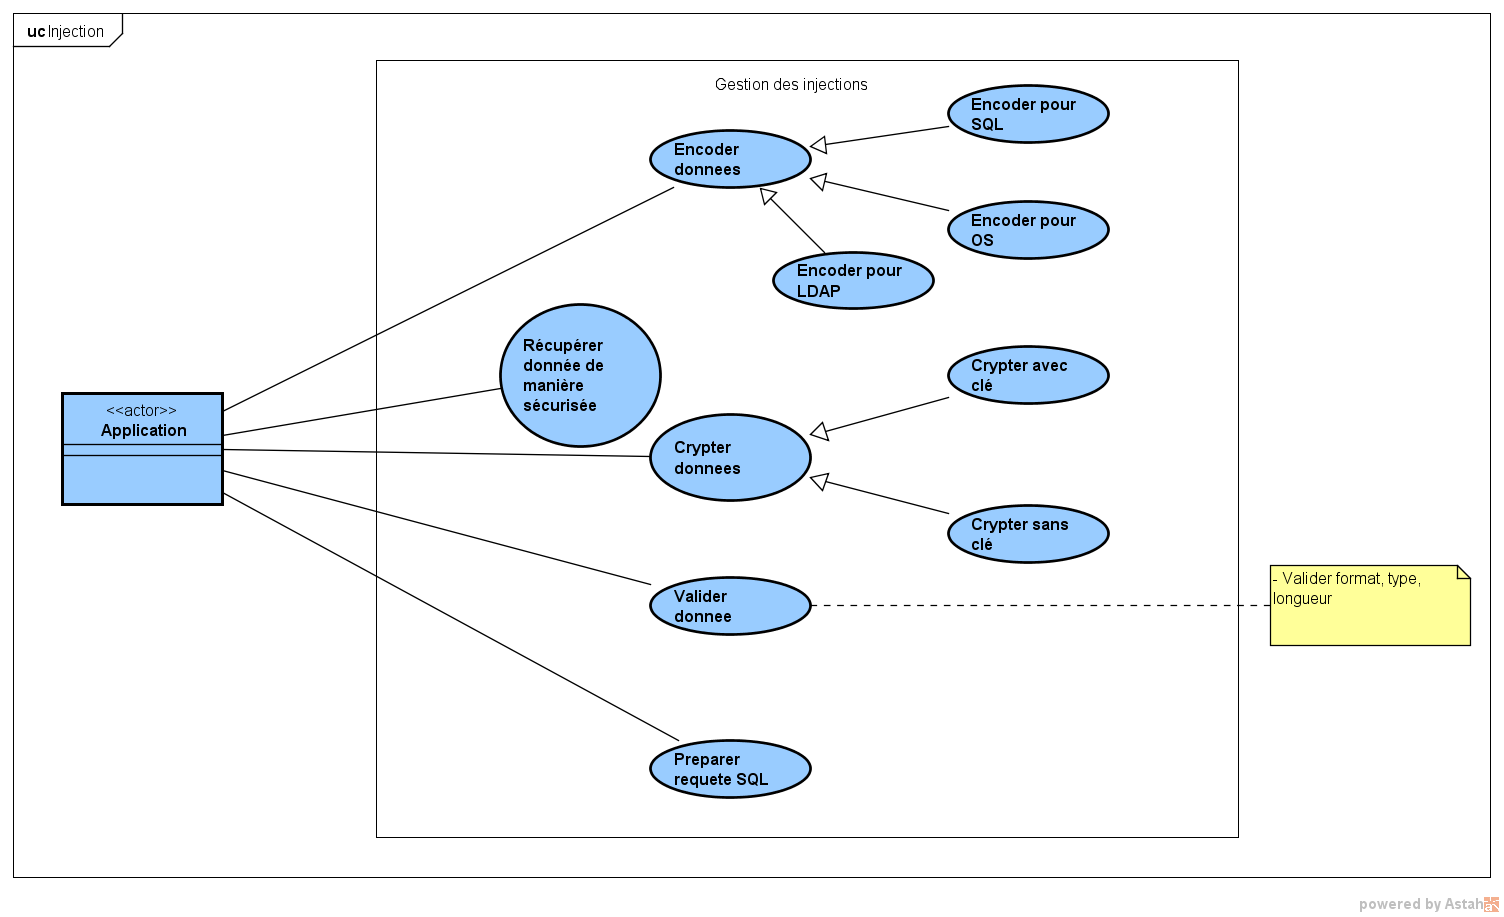
\includegraphics[height=0.30\textheight]{fig/Injection-use-case-diagram.png}}
	\end{minipage}
	\caption{Diagramme de cas d'utilisation du package "Gestion des injections"}
	\label{fig:7.2}
\end{figure}

\subsection{Package Gestion des violations de gestion d'authentification}

\subsubsection{Diagramme de cas d'utilisation}
Le diagramme de cas d'utilisation du package "Gestion des violations de gestion d'authentification" est representé ci-dessous. Il comprend les cas d'utilisation permettant à une application donnée de mitiger les risques de violations de gestion d'authentification.\\ 
\begin{figure}[H]
	\centering
	\begin{minipage}{12cm}
		\centering
		{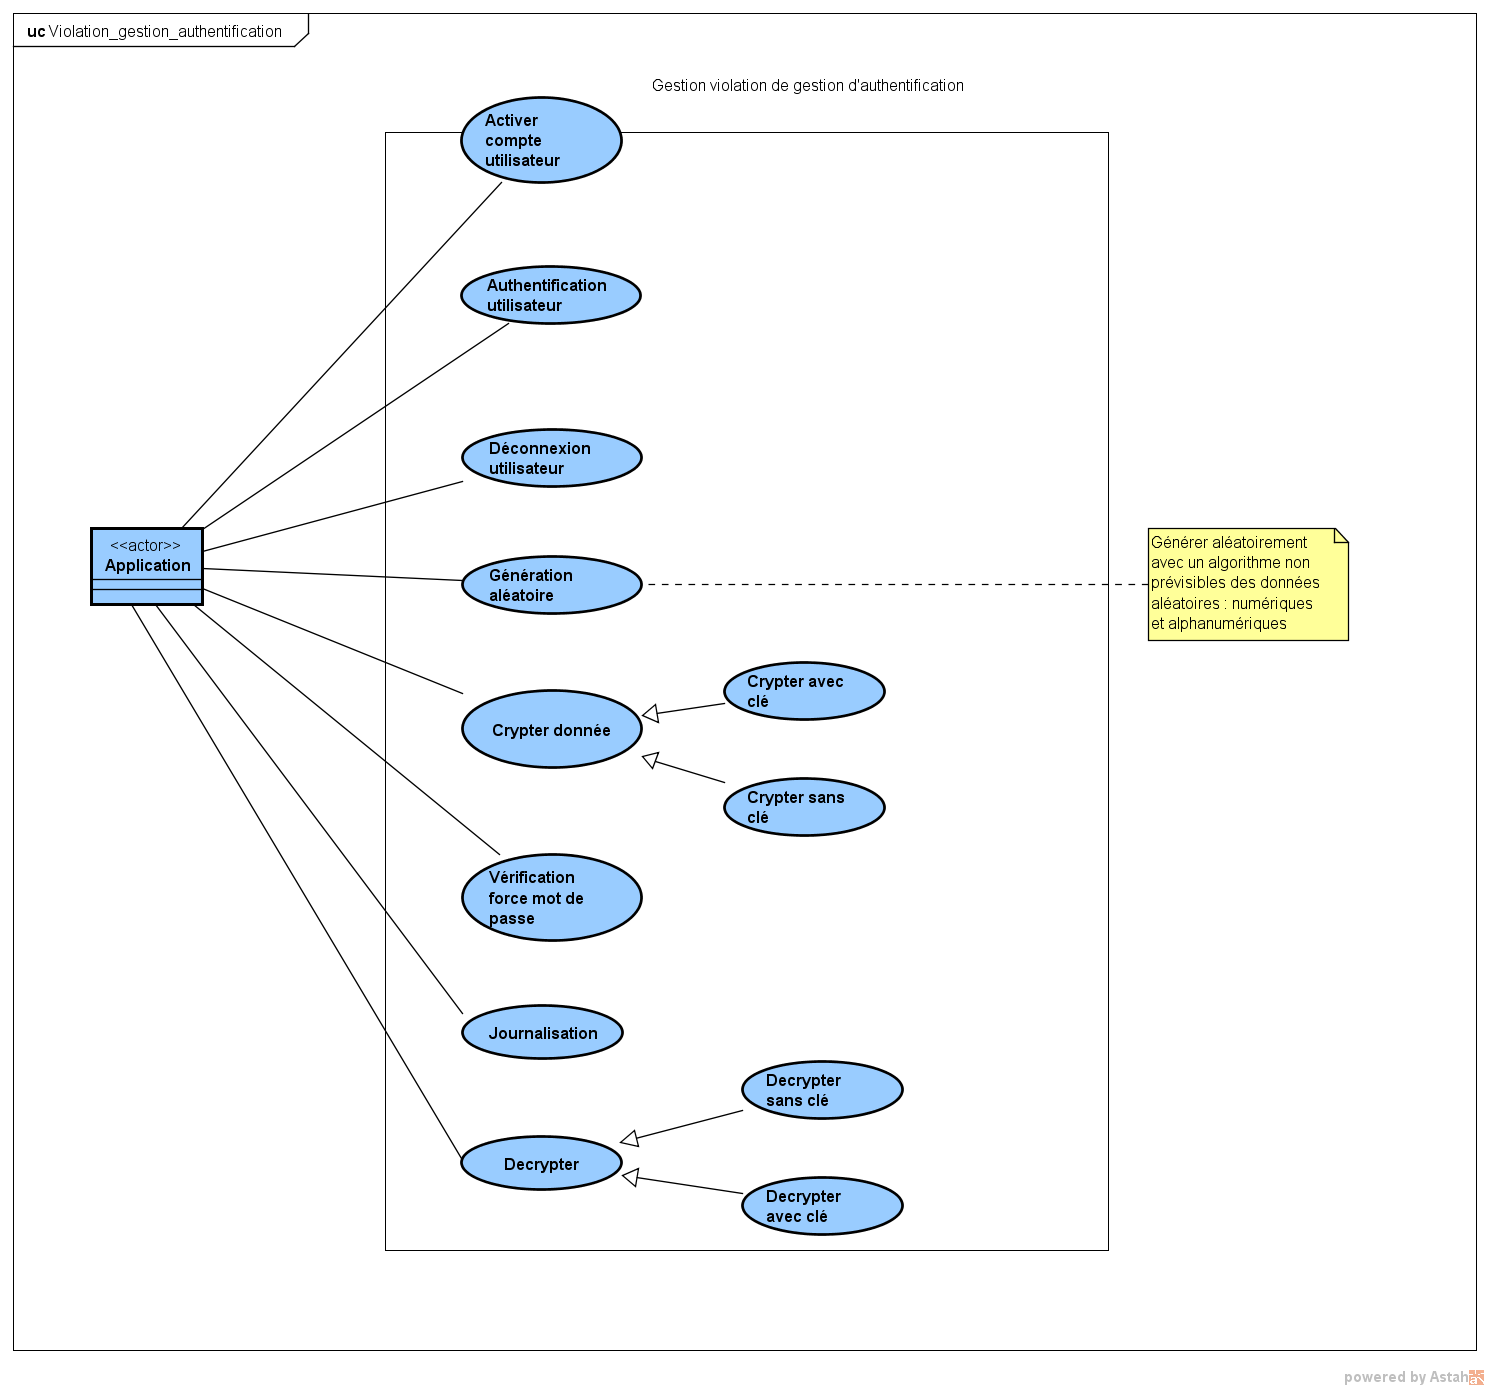
\includegraphics[height=0.30\textheight]{fig/Violation-gestion-authentification-use-case-diagram.png}}
	\end{minipage}
	\caption{Diagramme de cas d'utilisation du package "Gestion des violations de gestion d'authentification"}
	\label{fig:7.3}
\end{figure}

\subsection{Package Gestion des expositions de données sensibles}

\subsubsection{Diagramme de cas d'utilisation}
Le diagramme de cas d'utilisation du package "Gestion des expositions de données sensibles" est representé ci-dessous. Il comprend les cas d'utilisation permettant à une application donnée de mitiger les risques d'exposition de données sensibles.\\ 
\begin{figure}[H]
	\centering
	\begin{minipage}{12cm}
		\centering
		{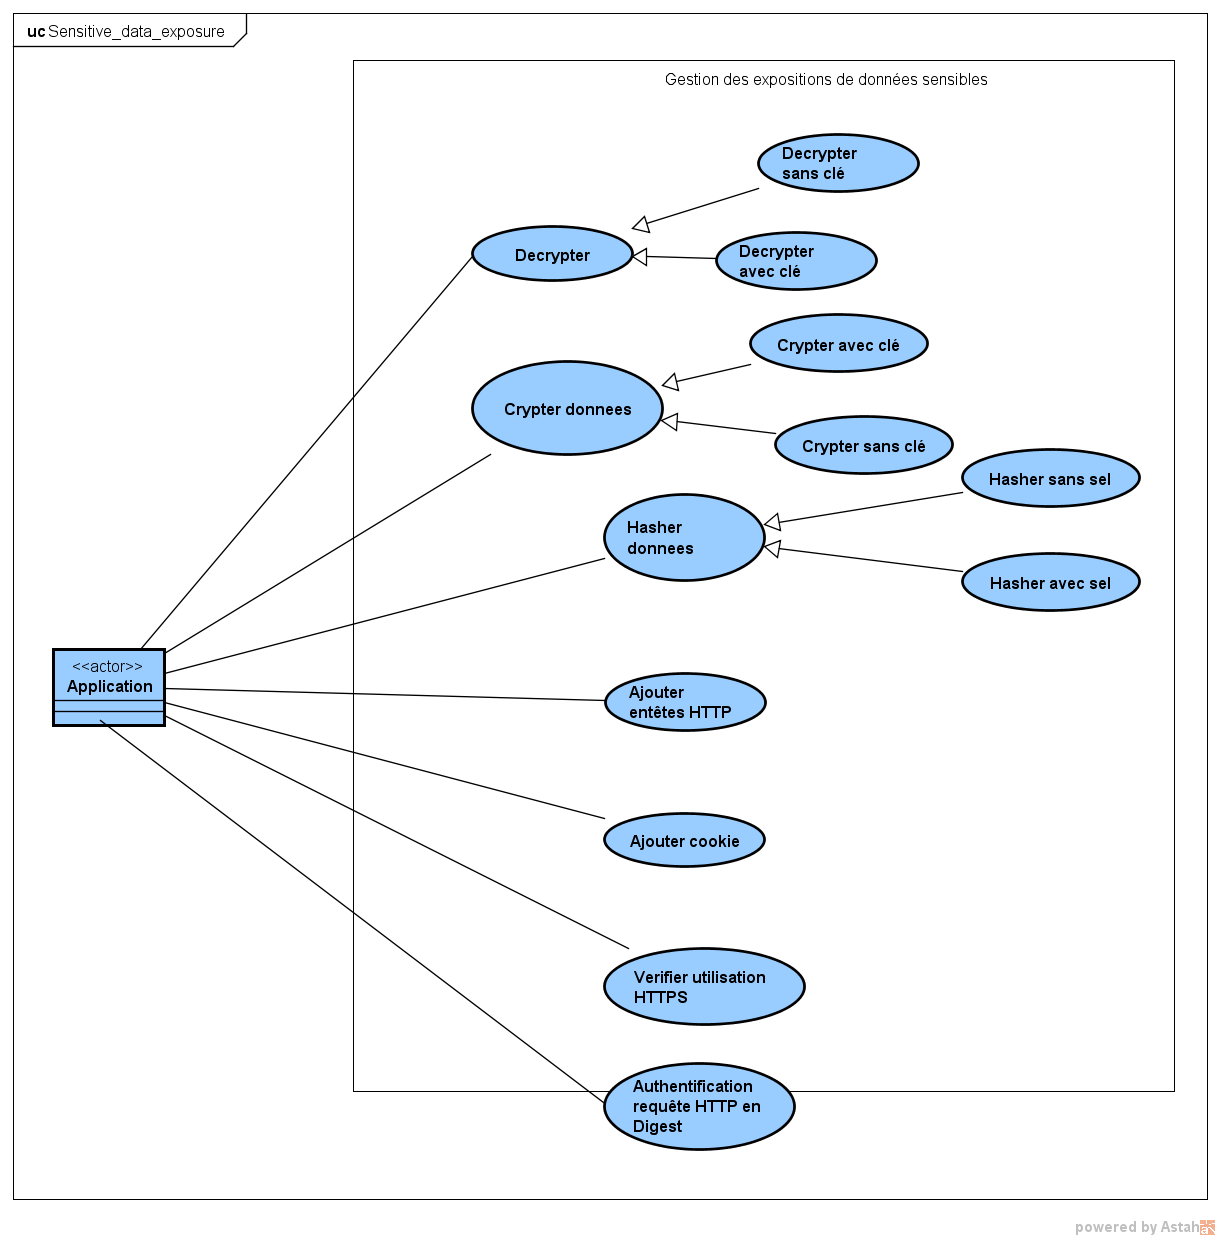
\includegraphics[height=0.30\textheight]{fig/Gestion-exposition-donnees-use-case-diagram.png}}
	\end{minipage}
	\caption{Diagramme de cas d'utilisation du package "Gestion des expositions de données sensibles"}
	\label{fig:7.4}
\end{figure}

\subsection{Package Gestion des attaques sur les entités XML externes}
\subsubsection{Diagramme de cas d'utilisation}
Le diagramme de cas d'utilisation du package "Gestion des attaques sur les entités XML externes" est representé ci-dessous. Il comprend les cas d'utilisation permettant à une application donnée de mitiger les risques découlant des attaques sur les entités XML externes.\\ 
\begin{figure}[H]
	\centering
	\begin{minipage}{12cm}
		\centering
		{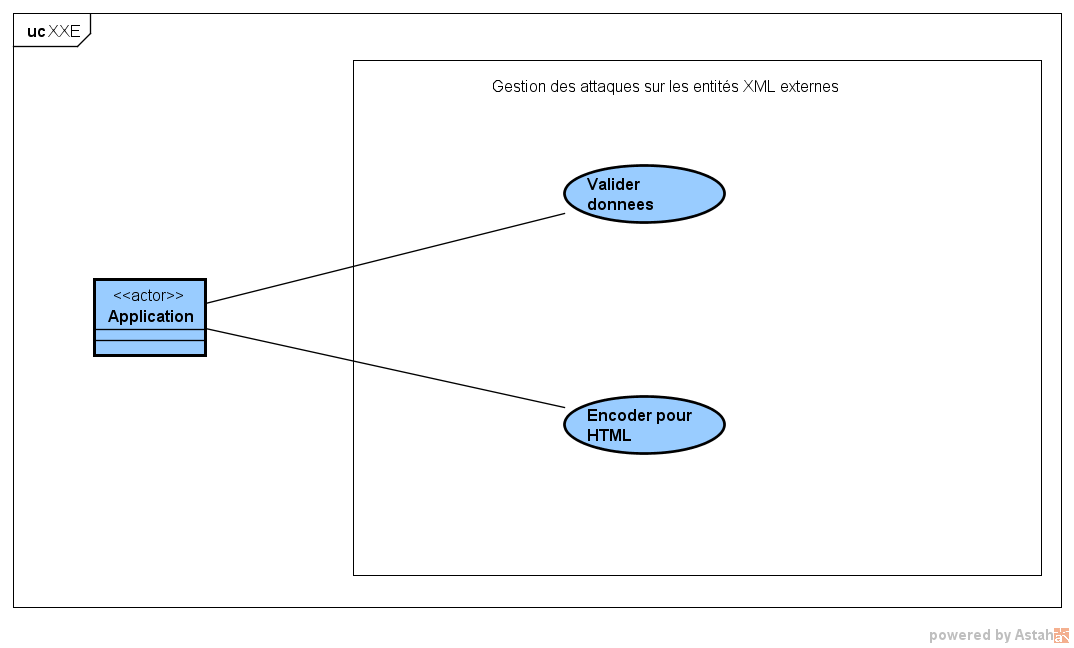
\includegraphics[height=0.30\textheight]{fig/XXE-use-case-diagram.png}}
	\end{minipage}
	\caption{Diagramme de cas d'utilisation du package "Gestion des attaques sur les entités XML externes"}
	\label{fig:7.5}
\end{figure}

\subsection{Package Gestion des violations de contrôle d'accès}
\subsubsection{Diagramme de cas d'utilisation}
Le diagramme de cas d'utilisation du package "Gestion des violations de contrôle d'accès" est représenté ci-dessous. Il comprend les cas d'utilisation permettant à une application donnée de mitiger les risques découlant des violations de contrôle d'accès.\\ 
\begin{figure}[H]
	\centering
	\begin{minipage}{12cm}
		\centering
		{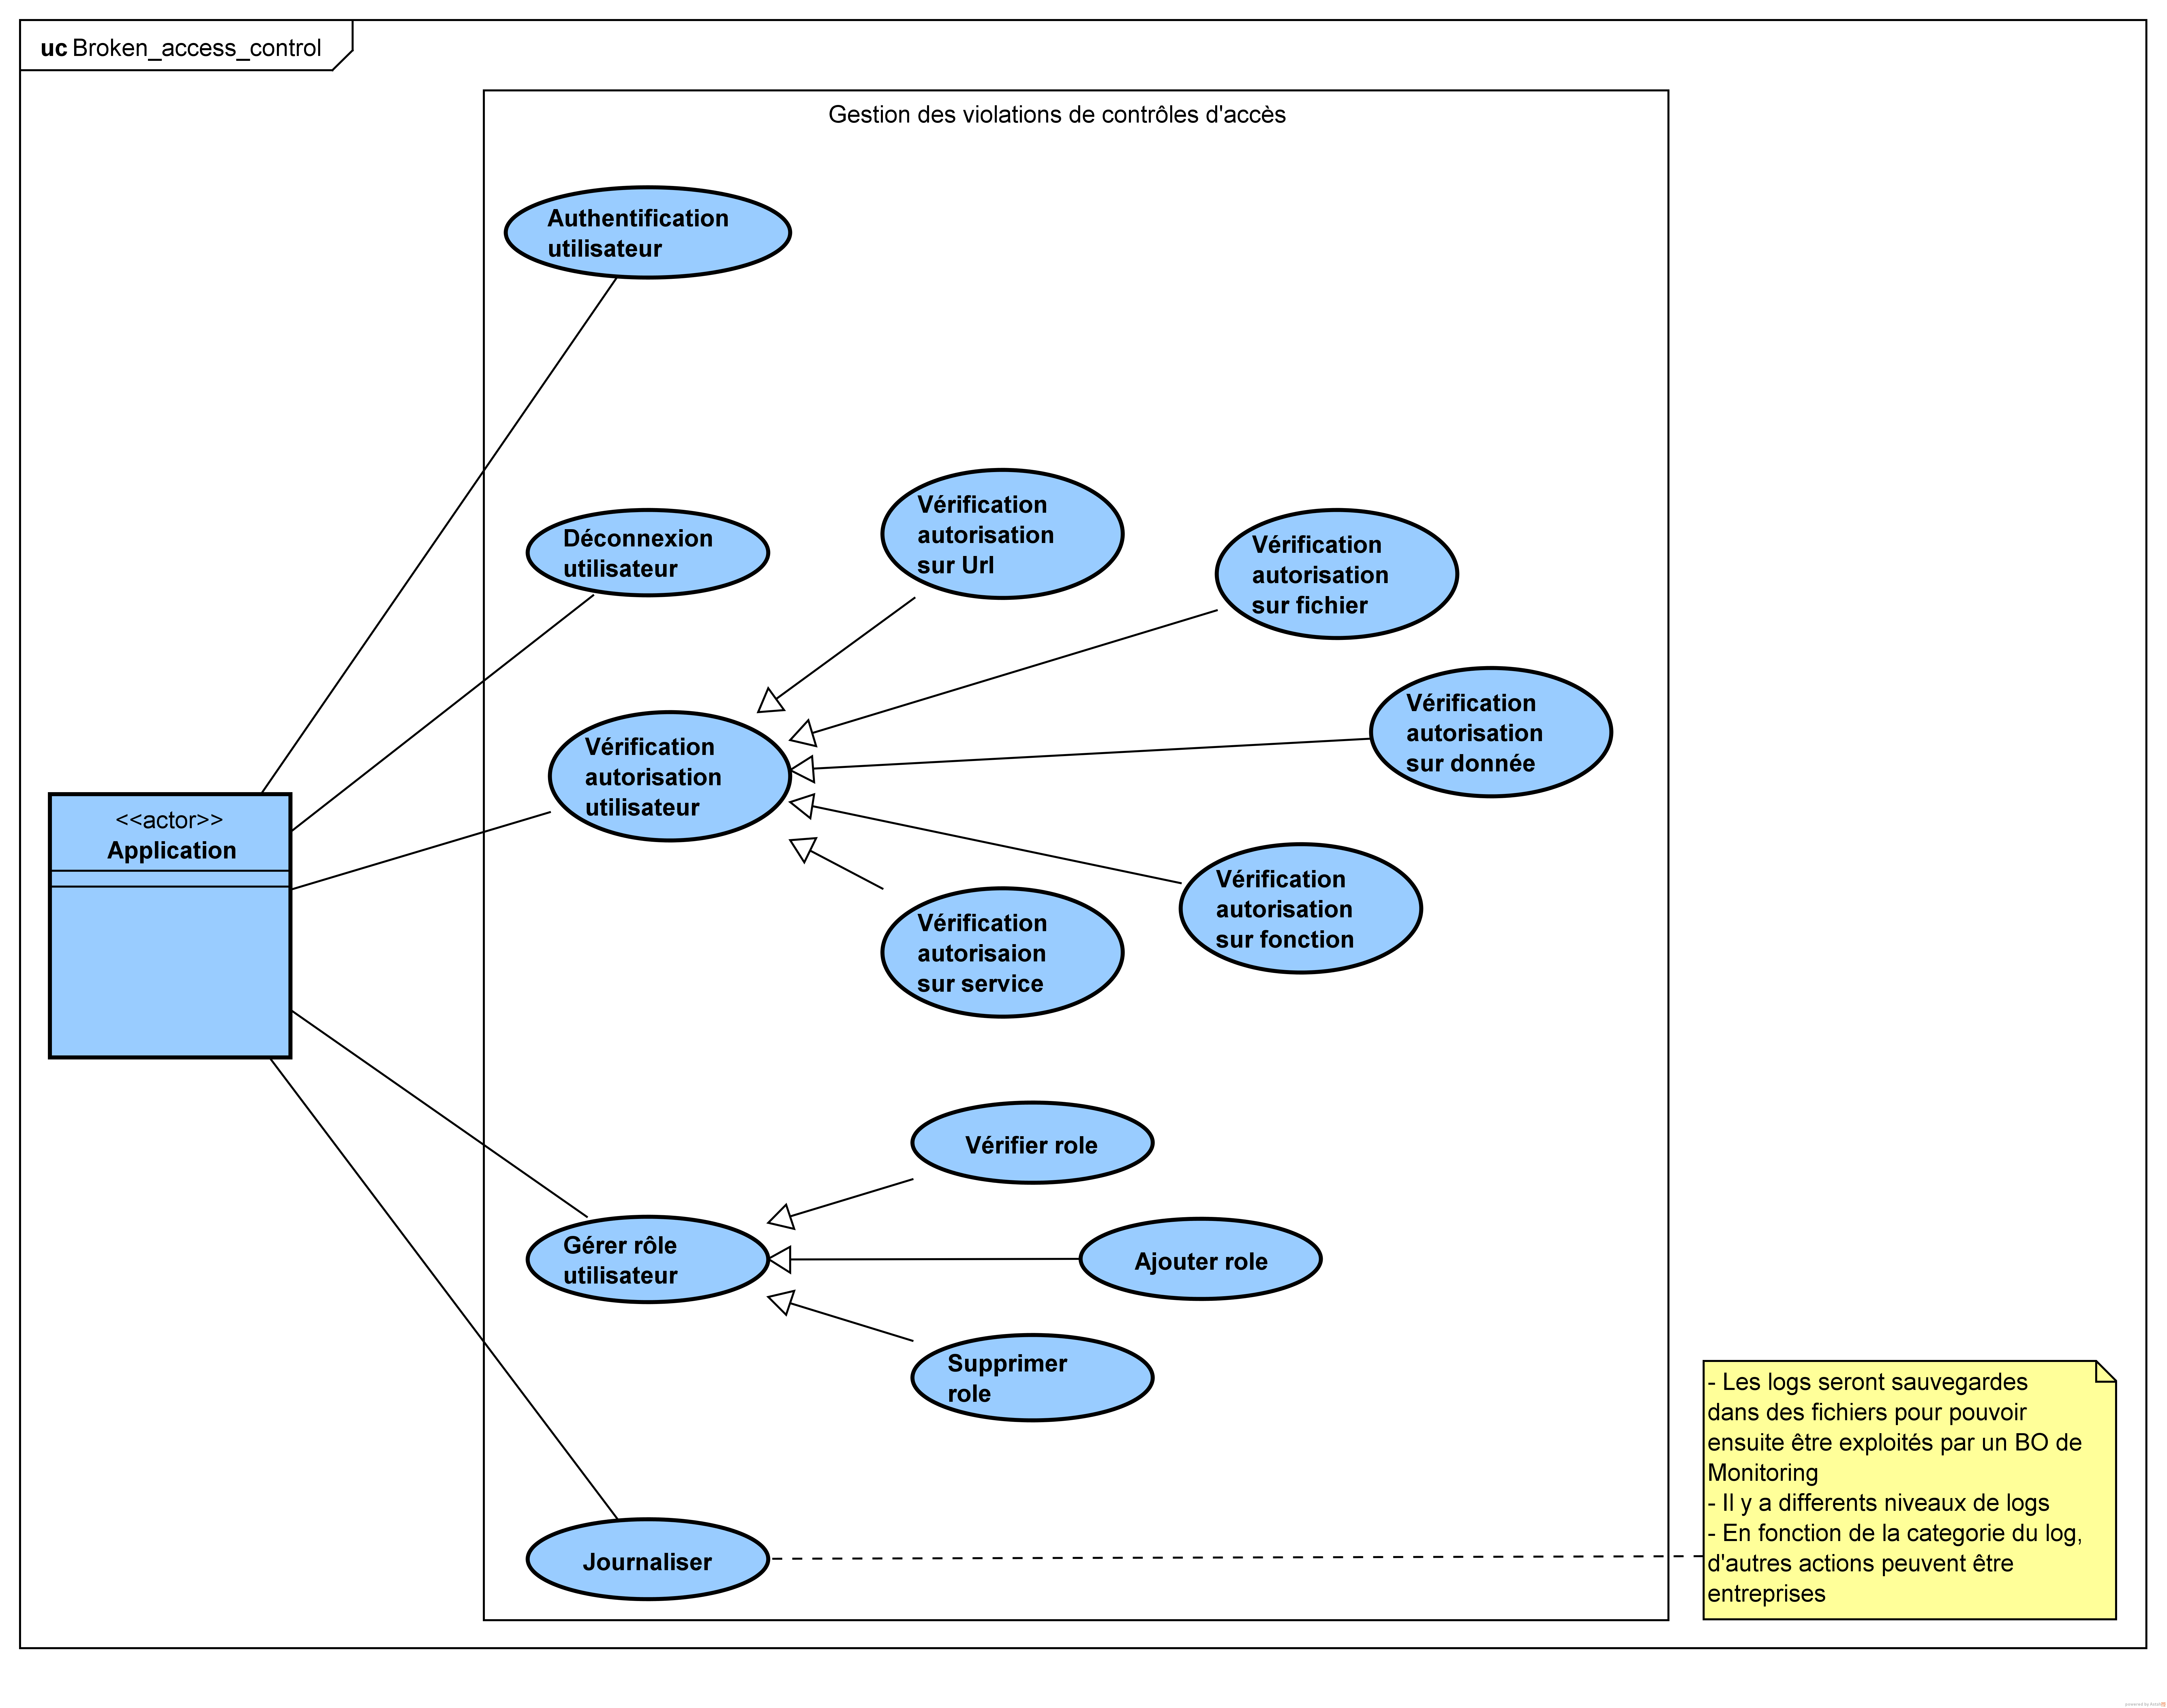
\includegraphics[height=0.30\textheight]{fig/Violation-controle-acces-use-case-diagram.png}}
	\end{minipage}
	\caption{Diagramme de cas d'utilisation du package "Gestion des violations de contrôle d'accès"}
	\label{fig:7.6}
\end{figure}

\subsection{Package Gestion des mauvaises configurations de sécurité}
\subsubsection{Diagramme de cas d'utilisation}
Le diagramme de cas d'utilisation du package "Gestion des mauvaises configurations de sécurité" est représenté ci-dessous. Il comprend les cas d'utilisation permettant à une application donnée de mitiger les risques de mauvaises configurations de sécurité.\\ 
\begin{figure}[H]
	\centering
	\begin{minipage}{12cm}
		\centering
		{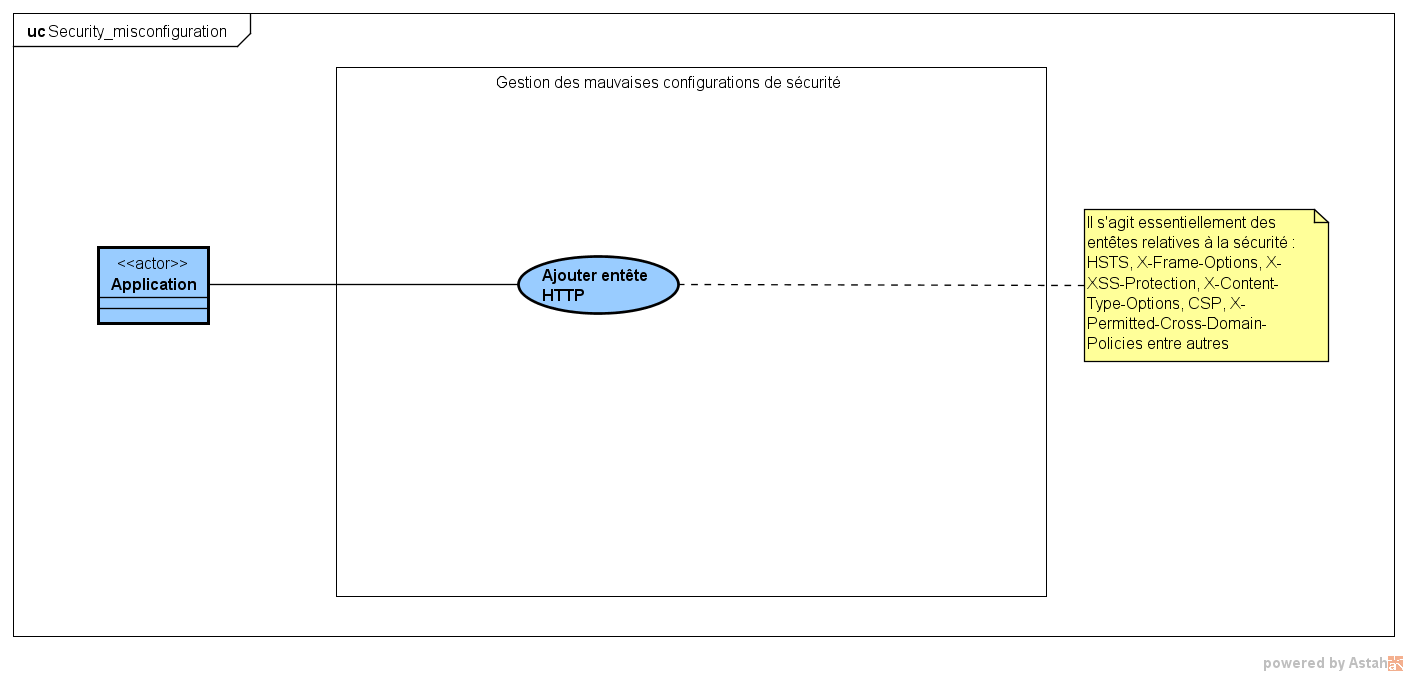
\includegraphics[height=0.30\textheight]{fig/Security_misconfiguration-use-case-diagram.png}}
	\end{minipage}
	\caption{Diagramme de cas d'utilisation du package "Gestion des mauvaises configurations de sécurité"}
	\label{fig:7.7}
\end{figure}

\subsection{Package Gestion des XSS }
\subsubsection{Diagramme de cas d'utilisation}
Le diagramme de cas d'utilisation du package "Gestion des XSS" est représenté ci-dessous. Il comprend les cas d'utilisation permettant à une application donnée de mitiger les attaques XSS.\\ 
\begin{figure}[H]
	\centering
	\begin{minipage}{12cm}
		\centering
		{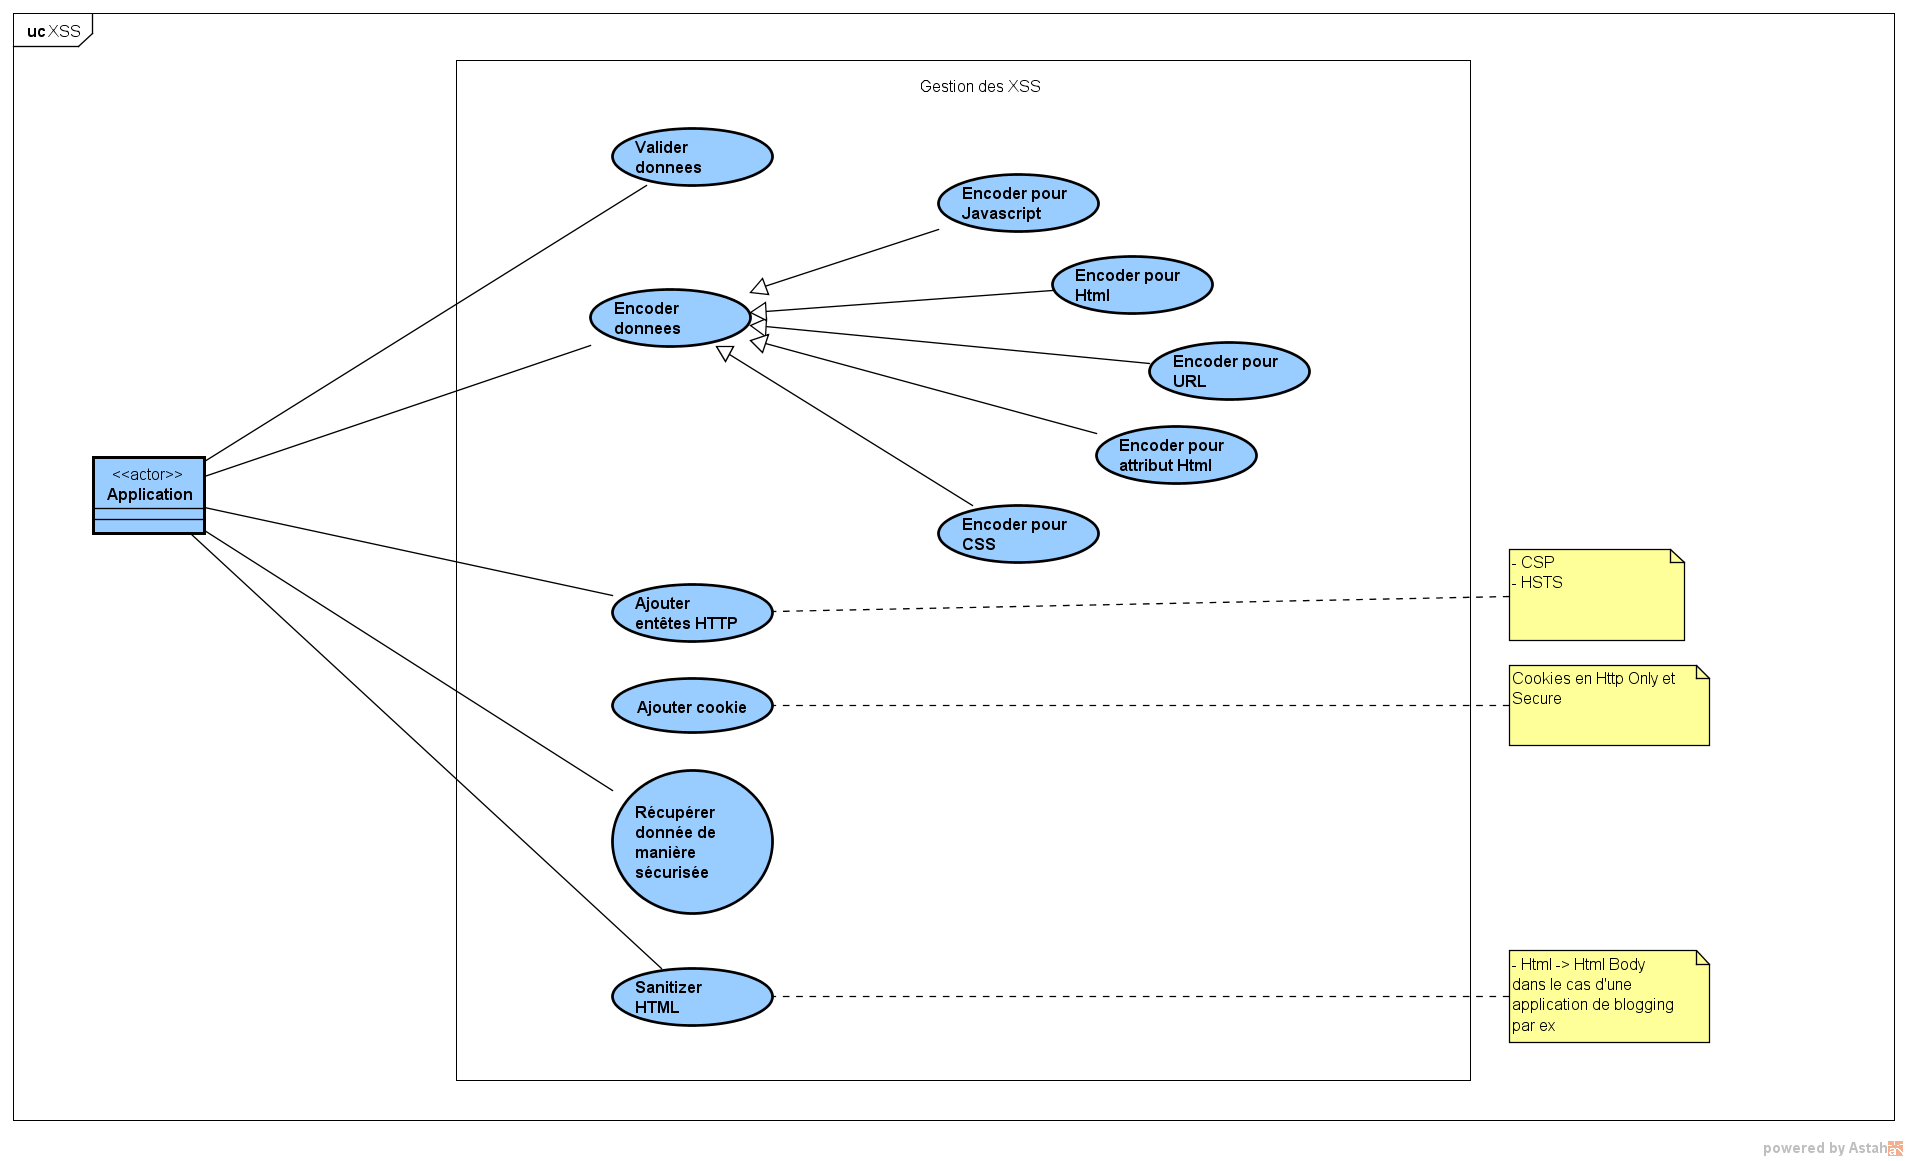
\includegraphics[height=0.30\textheight]{fig/XSS-use-case-diagram.png}}
	\end{minipage}
	\caption{Diagramme de cas d'utilisation du package "Gestion des XSS"}
	\label{fig:7.8}
\end{figure}

\subsection{Package Gestion des désérialisations non sécurisées}
\subsubsection{Diagramme de cas d'utilisation}
Le diagramme de cas d'utilisation du package "Gestion des désérialisations non sécurisées" est représenté ci-dessous. Il comprend les cas d'utilisation permettant à une application donnée de mitiger les risques de désérialisations non sécurisées.\\ 
\begin{figure}[H]
	\centering
	\begin{minipage}{12cm}
		\centering
		{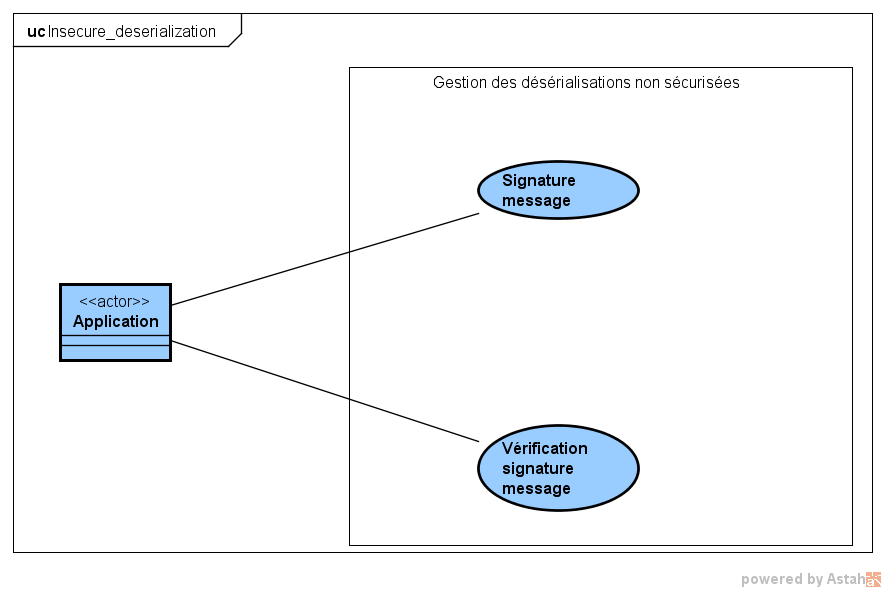
\includegraphics[height=0.30\textheight]{fig/Insecure_deserialization-use-case-diagram.png}}
	\end{minipage}
	\caption{Diagramme de cas d'utilisation du package "Gestion des désérialisations non sécurisées"}
	\label{fig:7.9}
\end{figure}

\subsection{Package Gestion des utilisations de composants vulnérables}
\subsubsection{Diagramme de cas d'utilisation}
Le diagramme de cas d'utilisation du package "Gestion des utilisations de composants vulnérables" est représenté ci-dessous. Il comprend les cas d'utilisation permettant à une application donnée de mitiger les risques découlant de l'utilisation de composants vulnérables.\\ 
\begin{figure}[H]
	\centering
	\begin{minipage}{12cm}
		\centering
		{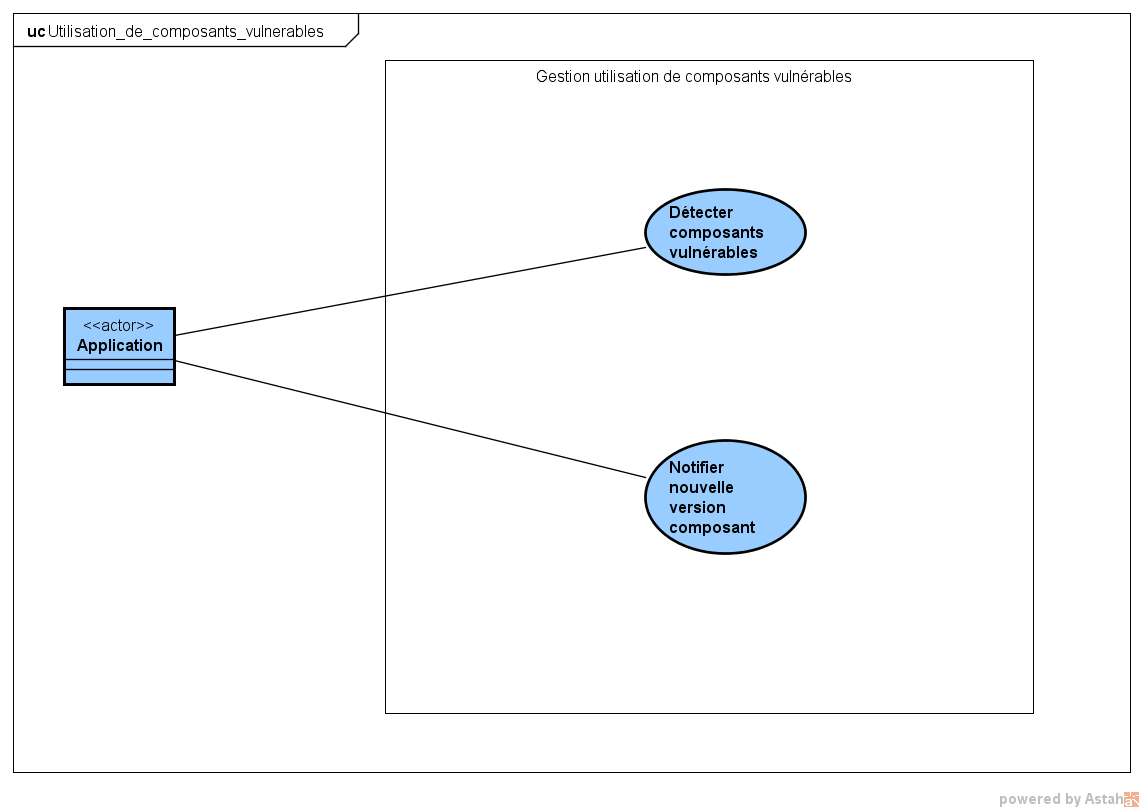
\includegraphics[height=0.30\textheight]{fig/Utilisation-composants-vulnerables-use-case-diagram.png}}
	\end{minipage}
	\caption{Diagramme de cas d'utilisation du package "Gestion des utilisations de composants vulnérables"}
	\label{fig:7.10}
\end{figure}

\subsection{Package Gestion de la journalisation et de la surveillance insuffisantes}
\subsubsection{Diagramme de cas d'utilisation}
Le diagramme de cas d'utilisation du package "Gestion de la journalisation et de la surveillance insuffisantes" est représenté ci-dessous. Il comprend les cas d'utilisation permettant à une application donnée de mitiger les risques de journalisation et de surveillance insuffisantes.\\ 
\begin{figure}[H]
	\centering
	\begin{minipage}{12cm}
		\centering
		{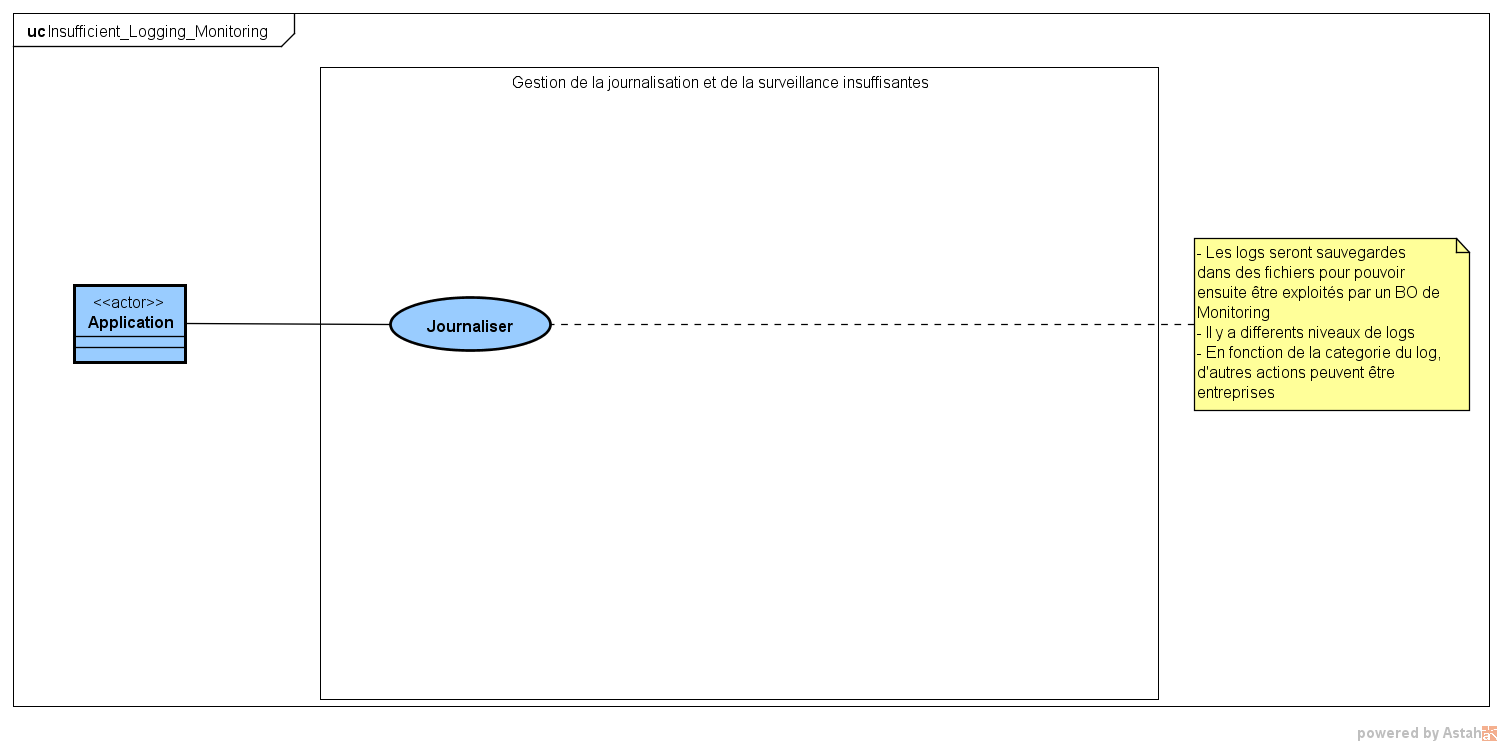
\includegraphics[height=0.30\textheight]{fig/Insufficient-logging-monitoring-use-case-diagram.png}}
	\end{minipage}
	\caption{Diagramme de cas d'utilisation du package "Gestion de la journalisation et de la surveillance insuffisantes"}
	\label{fig:7.11}
\end{figure}

\subsection{Système global}
Nous avons organisé les cas d'utilisation en packages, chaque package correspondant à la gestion d'un risque du Top 10, et cela pour des questions de lisibilité mais aussi pour des questions d'identification des fonctions de sécurité à mettre en place en adéquation avec le risque en question. Cependant, le système que nous devons mettre en place tourne autour de ces fonctions de sécurité. Il s'agit de mettre à la disposition des développeurs ces fonctions de sécurités. \\
En effet, certaines fonctions de sécurité recommandées pour un risque, peuvent aussi l'être pour d'autres.Par exemple, si l'on essaie de mitiger le risque de XSS, la meilleure façon de le faire est de mettre en place des fonctions permettant la validation des entrées ainsi que l'encodage des sorties que les développeurs peuvent facilement utiliser. Mais ces mêmes fonctions peuvent être utilisées pour se protéger de beaucoup  d’autres attaques. \\
Ainsi, nous nous concentrons maintenant sur ces fonctions de sécurité. Nous présenterons à la volée toutes les fonctionnalités attendues par les applications pour se protéger au moins des dix risques de sécurite présentes dans le Top 10.\\
Ci-dessous, nous avons le diagramme de cas d'utilisation global du système :
\begin{figure}[H]
	\centering
	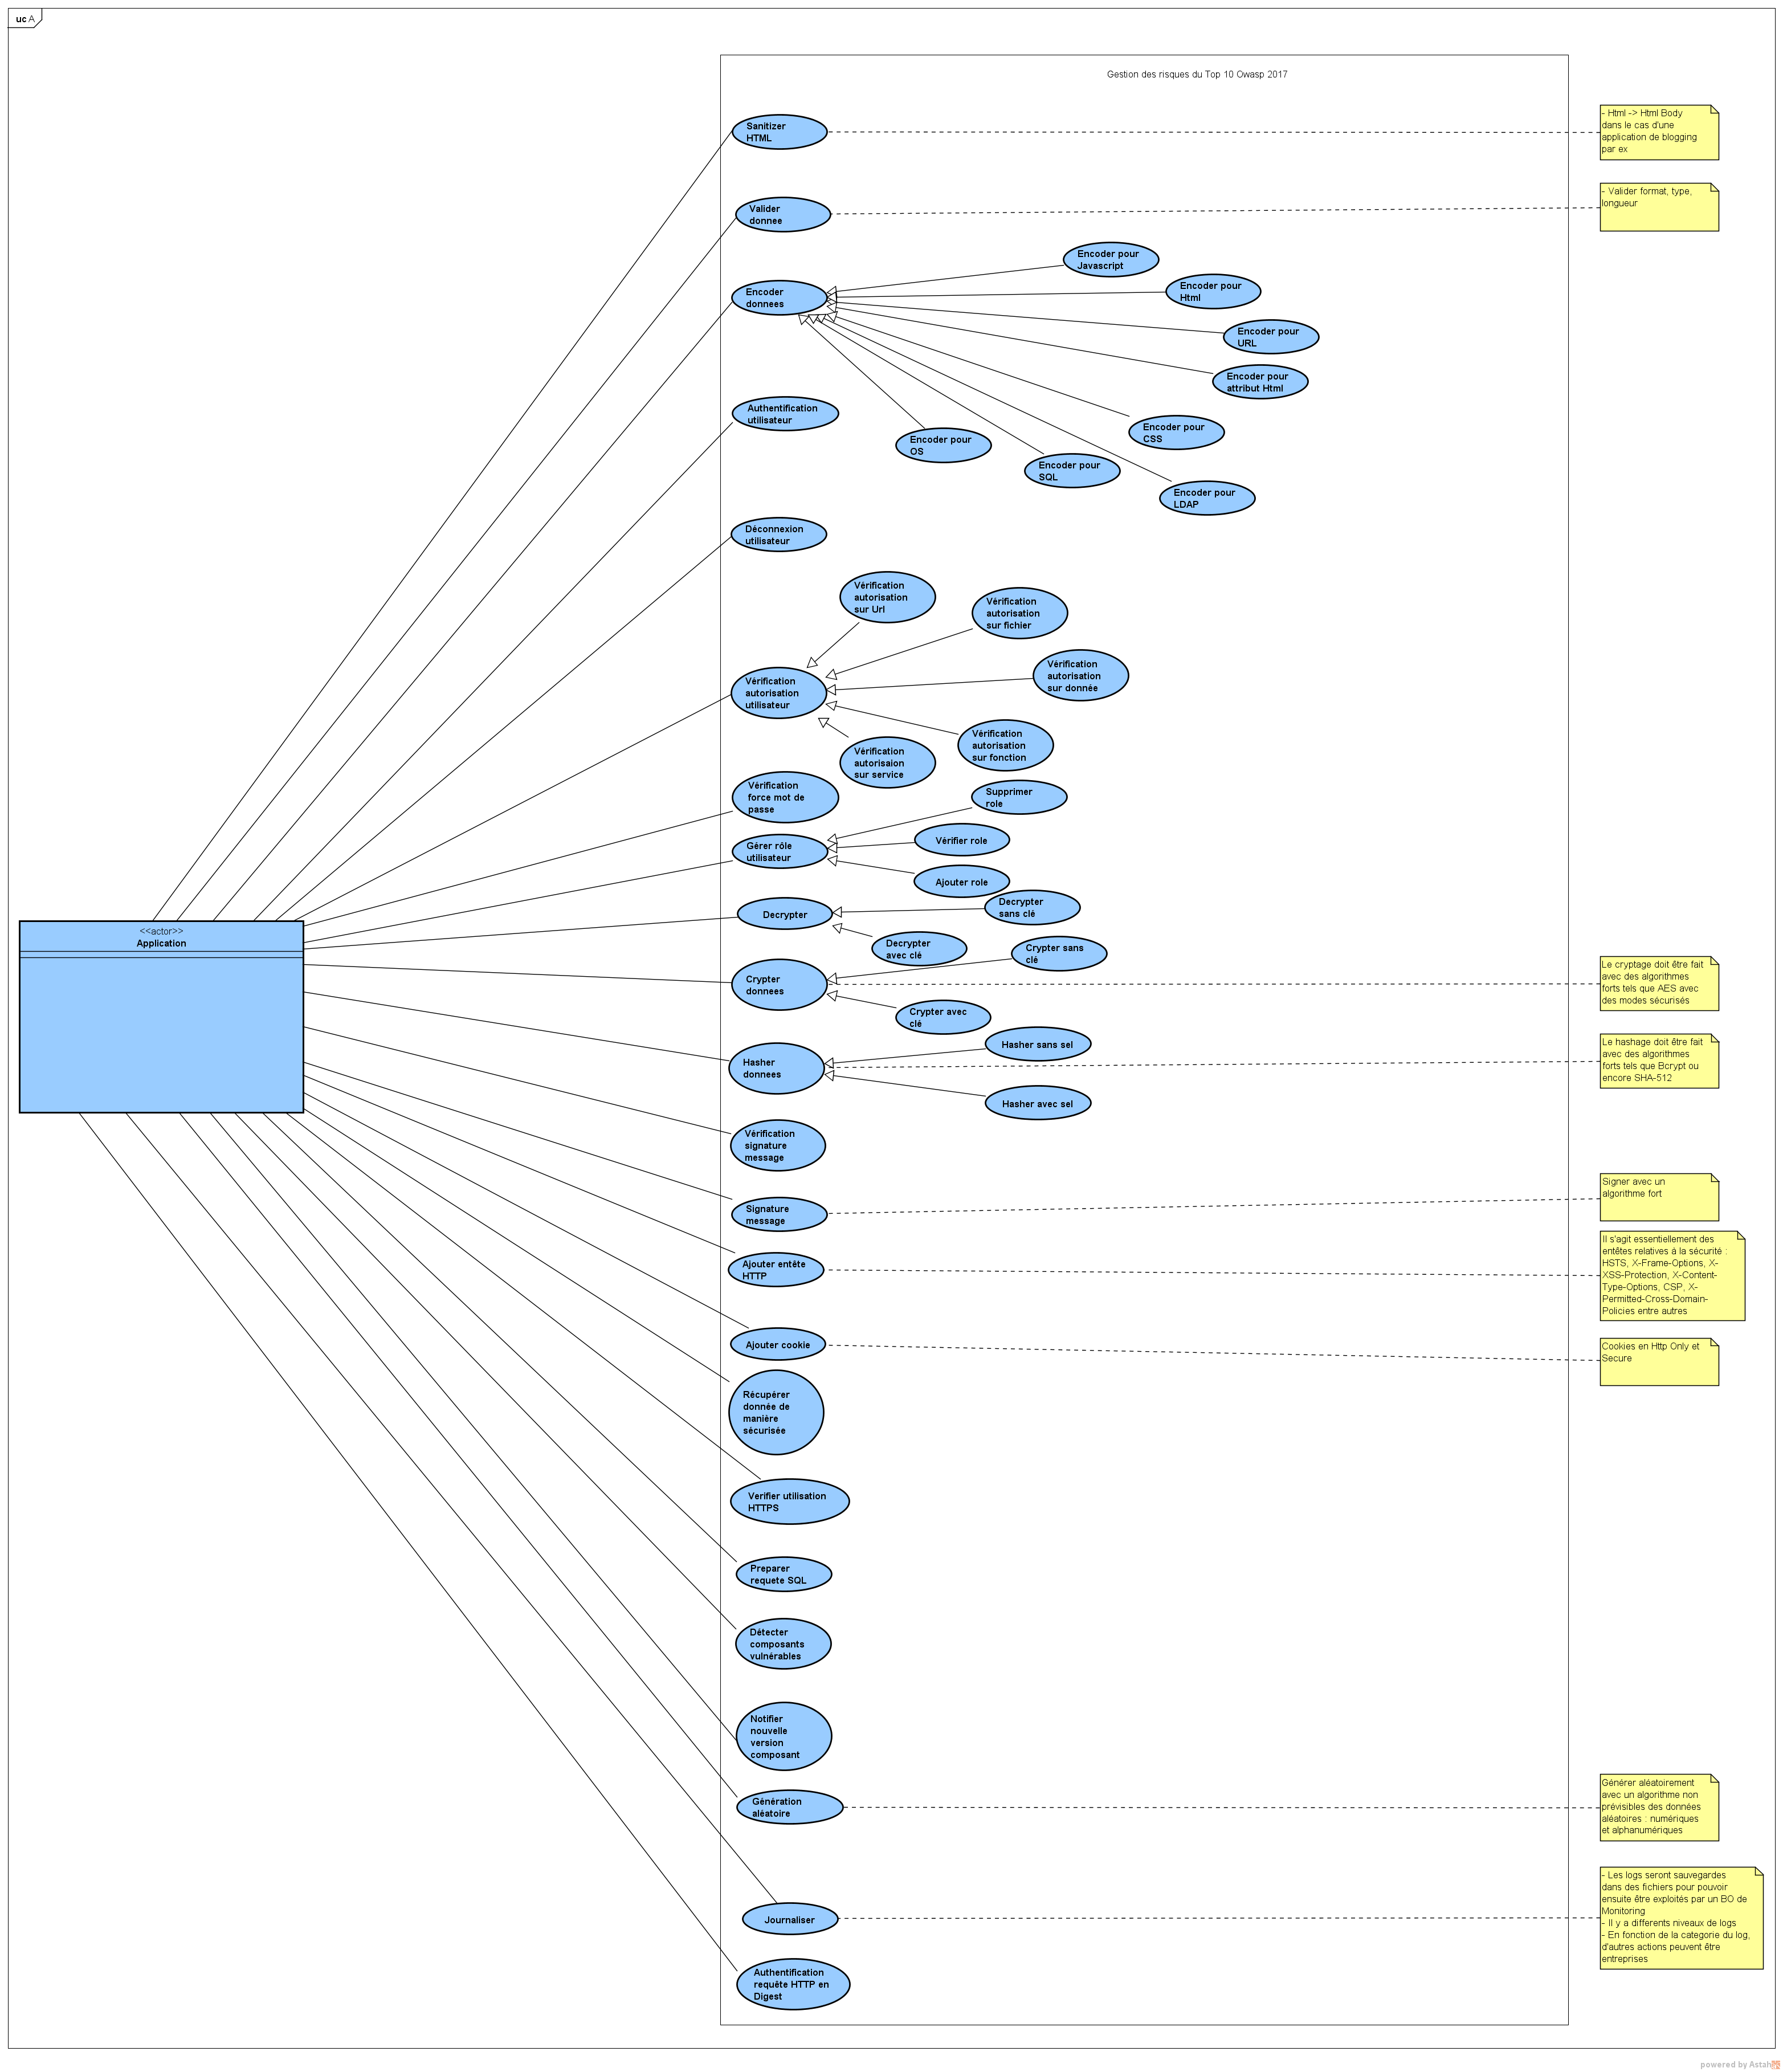
\includegraphics[width=1.0\textwidth,height=0.95\textheight]{fig/Global-use-case-diagram.png}
	\caption{Diagramme de cas d'utilisation global du système}
	\label{fig:7.12}
\end{figure}
Toutefois, cette représentation n'est pas non plus le meilleur car ne favorisant pas une bonne lisibilité. Ainsi, nous avons décidé pour des raisons de lisibilité de séparer ces fonctions en modules, chaque module comrenant les fonctions de sécurité de même nature.\\
Ainsi, nous avons les modules suivants :
- Module "Utilisateurs" comprenant les fonctions relatives aux utilisateurs ;\\
- Module "Cryptographie" comprenant les fonctions se rapportant à la cryptographie ; \\
- Module "Encodage" comprenant les fonctions d'encodage ; \\ 
- Module "Validation" regroupant les fonctions relatives à la validation ; \\
- Module "HTTP" regroupant les fonctions relatives aux paramètres HTTP;
- Module "Interpréteurs" regroupant les fonctions relatives aux interpréteurs;
- Module "Logging" regroupant les fonctions relatives à la journalisation ; \\
- Module "Gestion des composants" regroupant les fonctions relatives aux composants utilisés dans l'application.\\
Chaque module est un sous-sytème et sera représenté par un package. Cette séparation nous donne le diagramme de packages suivant :
\begin{figure}[H]
	\centering
	\includegraphics[height=0.5\textheight]{fig/S-Package-diagram.png}
	\caption{Diagramme de packages du système (réorganisé)"}
\end{figure}


\subsection{Sous-système "Utilisateurs"}

\subsubsection{Diagramme de cas d'utilisation}
\begin{figure}[H]
	\centering
	\begin{minipage}{12cm}
		\centering
		{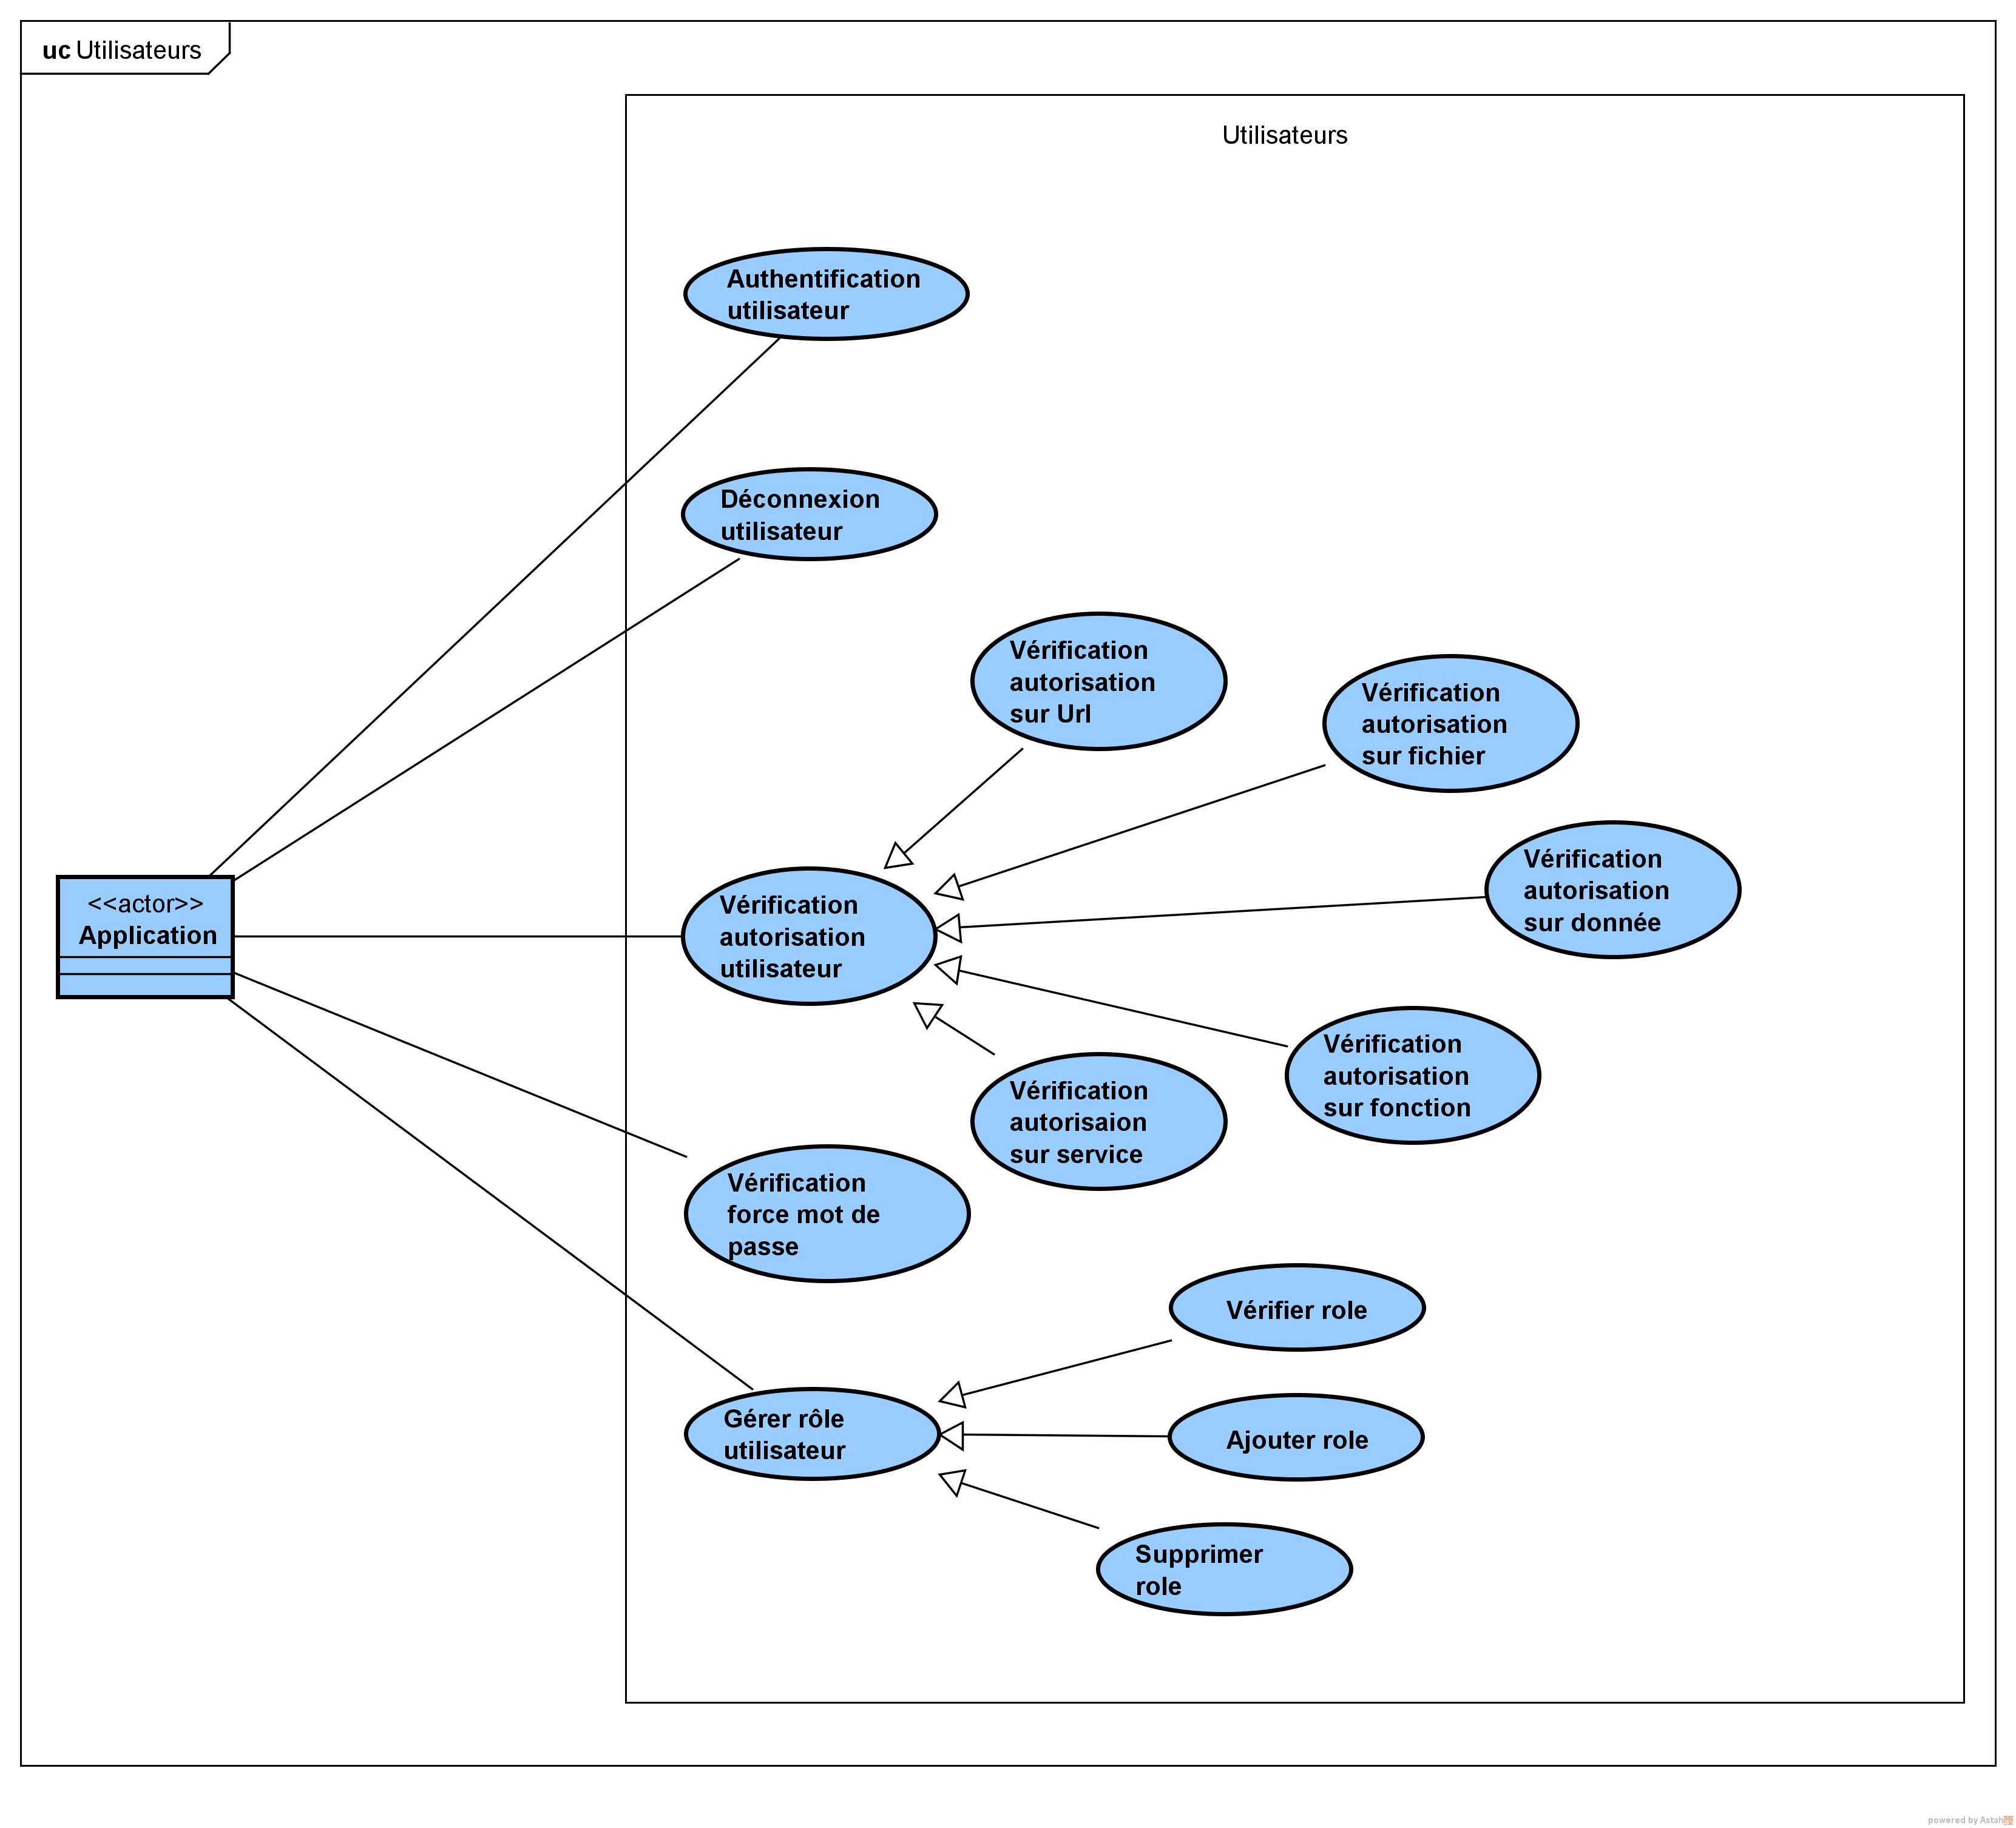
\includegraphics[height=0.35\textheight, width=1\textwidth]{fig/Utilisateurs-use-case-diagram.png}}
	\end{minipage}
	\caption{Diagramme de cas d'utilisation du sous-système "Utilisateurs"}
	\label{fig:7.13}
\end{figure}

\subsubsection{Cas d'utilisation "Authentification utilisateur"}
\textbf{\RIGHTarrow Description textuelle}\\
\underline{\underline{Sommaire d’identification}} \\
\textbf{Titre} : Authentification utilisateur\\
\textbf{Résumé} : Ce cas d’utilisation permet à une application d'authentifier un utilisateur.\\
\textbf{Acteur} : Application\\	
\textbf{Responsable} : Papa Latyr Mbodj\\
\underline{\underline{Description des scénarios}}\\
\textbf{Précondition(s)}
\begin{itemize}
	\item Aucune
\end{itemize}
\textbf{Scénario nominal}
\begin{enumerate}
	\item L'application donne une requête HTTP POST contenant nom d'utilisateur et mot de passe.
	\item Le système récupère l'utilisateur avec le nom d'utilisateur donné.
	\item Le système enregistre l'adresse IP de connexion.
	\item Le système s'assure que la requête est de type POST et que HTTPS est utilisé.
	\item Le système s'assure que l'utilisateur n'est pas expiré.
	\item Le système s'assure que l'utilisateur est activé.
	\item Le système s'assure que l'utilisateur n'est pas bloqué.
	%\item Le système s'assure que le délai d'inactivité de l'utilisateur n'est pas atteint.
	%\item Le système s'assure que la session de l'utilisateur n'est pas expirée.
	\item Le système déconnecte l'utilisateur.
	\item Le système hashe le mot de passe donné et le compare avec celui de l'utilisateur récupéré précédemment.
	\item Le système crée une nouvelle session pour l'utilisateur et l'enregistre.
	\item Le système enregistre la date et l'heure de connexion 
	\item Le système enregistre l'adresse IP de l'hôte ayant envoyé la requête.
	Le système met à jour l'état de connexion de l'utilisateur
	\item Le système journalise la connexion de l'utilisateur.
	\item Le système retourne l'utilisateur modifié.
\end{enumerate}
%\textbf{Enchainements alternatif(s)}\\
\textbf{Enchainements d’erreur}\\
\textit{E1 : Utilisateur avec nom d'utilisateur donné inexistant}\\
L’enchaînement E1 démarre au point 2 du scénario nominal.
\begin{itemize}
	\item[3.] Le système journalise l'échec de la connexion avec le message "Login ou mot de passe incorrect".
	\item[4.] Le système produit une exception avec le même message.
	\item[5.] Le système refuse la connexion; le cas d'utilisation se termine en échec.
\end{itemize}
\textit{E2 : Requête pas de type POST ou HTTPS non utilisé}\\
L’enchaînement E2 démarre au point 4 du scénario nominal.
\begin{itemize}
	\item[5.] Le système met à jour la date et l'heure de la dernière connexion échouée de l'utilisateur.
	\item[6.] Le système incrémente le nombre de tentatives de connexion échouées pour cet utilisateur.
	\begin{itemize}
		\item[6.a.] Nombre maximal de tentatives de connexions échouées atteint ou dépassé : 
		\begin{itemize}
			\item[6.a.1.] Le système bloque l'utilisateur.
			\item[6.a.2.] Le système journalise le blocage de l'utilisateur avec le message "Utilisateur bloqué" avec le nom de l'utilisateur.
			\item[6.a.3.] Le système produit une exception avec le même message.
		\end{itemize}	
		\item[6.b.] Nombre maximal de tentatives de connexions échouées non atteint :
		\begin{itemize}
			\item[6.b.1] Le système journalise l'échec de la connexion avec le message "Tentative de connexion avec une requête non sécurisée".
			\item[6.b.2] Le système produit une exception avec le même message.
		\end{itemize}	
	\end{itemize}
	\item[7.] Le système refuse la connexion; le cas d'utilisation se termine en échec.
\end{itemize}
\textit{E3 : Utilisateur expiré}\\
L’enchaînement E3 démarre au point 5 du scénario nominal.
\begin{itemize}
	\item[6.] Le système journalise l'échec de la connexion avec le message "Utilisateur expiré" avec le nom de l'utilisateur.
	\item[7.] Le système produit une exception avec le même message.
	\item[8.] Le système refuse la connexion; le cas d'utilisation se termine en échec.
\end{itemize}
\textit{E4 : Utilisateur non activé}\\
L’enchaînement E4 démarre au point 6 du scénario nominal.
\begin{itemize}
	\item[7.] Le système journalise l'échec de la connexion avec le message "Utilisateur inactif" avec le nom de l'utilisateur.
	\item[8.] Le système produit une exception avec le même message.
	\item[9.] Le système refuse la connexion; le cas d'utilisation se termine en échec.
\end{itemize}
\textit{E5 : Utilisateur bloqué}\\
L’enchaînement E5 démarre au point 7 du scénario nominal.
\begin{itemize}
	\item[8.] Le système met à jour la date et l'heure de la dernière connexion échouée de l'utilisateur.
	\item[9.] Le système incrémente le nombre de tentatives de connexion échouées pour cet utilisateur.
	\begin{itemize}
		\item[10.a.] Nombre maximal de tentatives de connexions échouées atteint ou dépassé : 
		\begin{itemize}
			\item[10.a.1.] Le système bloque l'utilisateur.
			\item[10.a.2.] Le système journalise le blocage de l'utilisateur avec le message "Utilisateur bloqué" avec le nom de l'utilisateur.
			\item[10.a.3.] Le système produit une exception avec le même message.
			\item[10.a.4.] Le système refuse la connexion; le cas d'utilisation se termine en échec.
		\end{itemize}
	\end{itemize}
\end{itemize}
%\textit{E6 : Délai d'inactivité de l'utilisateur atteint}\\
%L’enchaînement E6 démarre au point 8 du scénario nominal.
%\begin{itemize}
%	\item[9.] Le système met à jour la date et l'heure de dernière connexion échouée de l'utilisateur.
%	\item[10.] Le système déconnecte l'utilisateur.
%\item[11.] Le système journalise l'échec de la connexion avec le message "Délai d'inactivité atteint" avec le nom de l'utilisateur.
%	\item[12.] Le système produit une exception avec le même message.
%	\item[13.] Le système refuse la connexion; le cas d'utilisation se termine en échec.
%\end{itemize}
%\textit{E7 : Session utilisateur expirée}\\
%L’enchaînement E7 démarre au point 9 du scénario nominal.
%\begin{itemize}
%	\item[8.] Le système met à jour la date et l'heure de dernière connexion échouée de l'utilisateur.
%	\item[9.] Le système déconnecte l'utilisateur.
%	\item[10.] Le système journalise l'échec de la connexion avec le message "Session expirée" avec le nom de l'utilisateur.
%	\item[11.] Le système produit une exception avec le même message.
%	\item[12.] Le système refuse la connexion; le cas d'utilisation se termine en échec.
%\end{itemize}
\textit{E8 : Mot de passe erroné}\\
L’enchaînement E8 démarre au point 9 du scénario nominal.
\begin{itemize}
	\item[12.] Le système met à jour la date et l'heure de dernière connexion échouée de l'utilisateur.
	\item[13.] Le système incrémente le nombre de tentatives de connexion échouées pour cet utilisateur.
	\begin{itemize}
			\item[13.a.] Nombre maximal de tentatives de connexions échouées atteint :
			\begin{itemize}
				\item[13.a.1.] Le système bloque l'utilisateur.
				\item[13.a.2.] Le système journalise le blocage de l'utilisateur avec le message "Utilisateur bloqué" avec le nom de l'utilisateur.
				\item[13.a.3.] Le système produit une exception avec le même message.
				\item[13.a.4.] Le système refuse la connexion; le cas d'utilisation se termine en échec.
			\end{itemize}
			\item[13.b.] Nombre maximal de tentatives de connexions échouées non atteint :
			\begin{itemize}
				\item[13.b.1] Le système journalise l'échec de la connexion avec le message "Login ou mot de passe incorrect".
				\item[13.b.2] Le système produit une exception avec le même message. en échec.
			\end{itemize}
	\end{itemize}
	\item[14.] Le système refuse la connexion; le cas d'utilisation se termine en échec.
\end{itemize}
\textbf{Post-condition(s)}
\begin{itemize}
	\item L’utilisateur en question est authentifié sur l'application.
\end{itemize}
\underline{\underline{Exigences non fonctionnelles}}
\begin{itemize}
	\item L’application doit être hébergée sur un serveur protégé par un firewall anti DDoS.\\
\end{itemize}

\textbf{\RIGHTarrow Diagramme d'activités}\\
\begin{figure}[H]
	\centering
	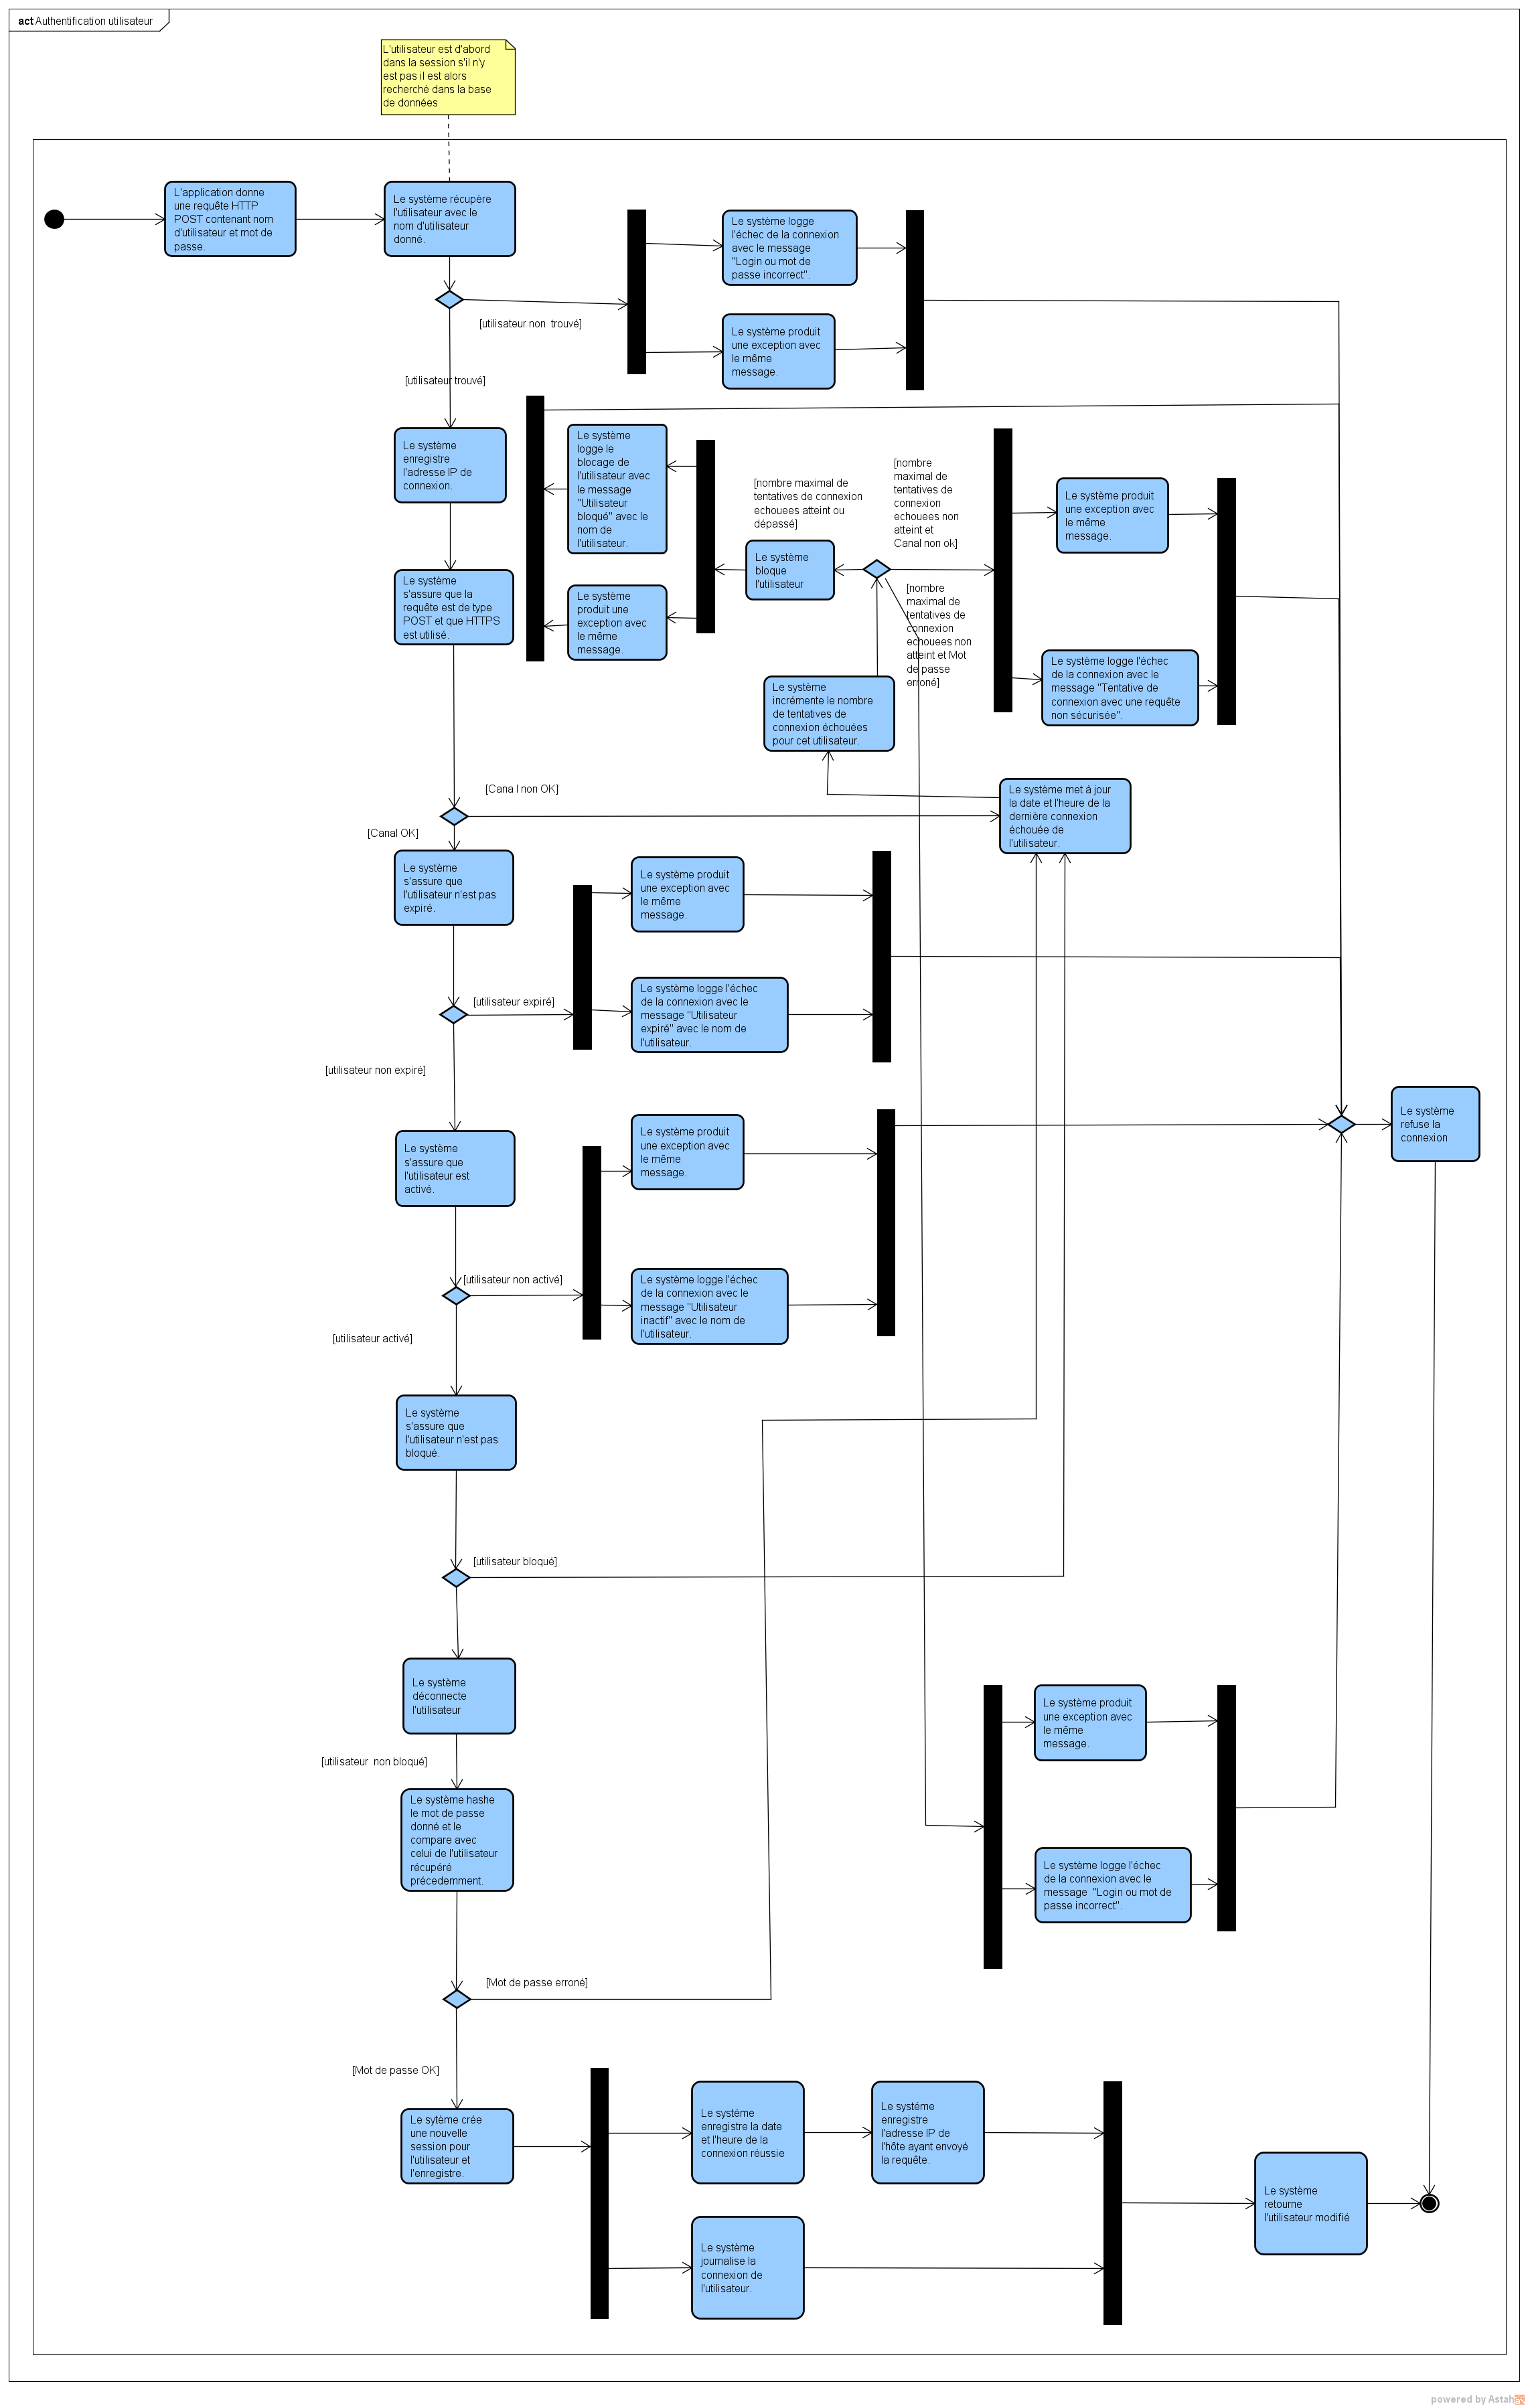
\includegraphics[width=1.0\textwidth,height=0.95\textheight]{fig/Authentification-utilisateur-activity-diagram.png}
	\caption{Diagramme d'activités du cas "Authentification utilisateur"}
\end{figure}

\subsubsection{Cas d'utilisation "Déconnexion utilisateur"}
\textbf{\RIGHTarrow Description textuelle}\\
\underline{\underline{Sommaire d’identification}} \\
\textbf{Titre} : Déconnexion utilisateur\\
\textbf{Résumé} : Ce cas d’utilisation permet à une application de déconnecter un utilisateur.\\
\textbf{Acteur} : Application\\	
\textbf{Responsable} : Papa Latyr Mbodj\\
\underline{\underline{Description des scénarios}}\\
\textbf{Précondition(s)}
\begin{itemize}
	\item Aucune
\end{itemize}
\textbf{Scénario nominal}
\begin{enumerate}
	\item Le système supprime le cookie "Se rappeler de moi".
	\item Le système invalide la session contenue dans la requête courante.
	\item Le système supprime le cookie contenant l'identificateur de session.
	\item Le système met à jour l'état de connexion de l'utilisateur.
	\item Le système journalise la déconnexion de l'utilisateur.
\end{enumerate}
%\textbf{Enchainements alternatif(s)}\\
\textbf{Post-condition(s)}
\begin{itemize}
	\item L’utilisateur en question est déconnecté de l'application.
\end{itemize}

\subsubsection{Cas d'utilisation "Vérification force mot de passe"}
\textbf{\RIGHTarrow Description textuelle}\\
\underline{\underline{Sommaire d’identification}} \\
\textbf{Titre} : Vérification force mot de passe\\
\textbf{Résumé} : Ce cas d’utilisation permet à une application de vérifier qu'un nouveau mot de passe est fort.\\
\textbf{Acteur} : Application\\	
\textbf{Responsable} : Papa Latyr Mbodj\\
\underline{\underline{Description des scénarios}}\\
\textbf{Précondition(s)}
\begin{itemize}
	\item Aucune
\end{itemize}
\textbf{Scénario nominal}
\begin{enumerate}
	\item L'application donne le login, l'ancien mot de passe et le nouveau mot de passe.
	\item Le système s'assure que le nouveau mot de passe n'est pas nul.
	\item Le système s'assure que le nouveau mot de passe ne correspond pas au login.
	\item Le système s'assure que le nouveau mot de passe ne contient pas une partie de l'ancien mot de passe (3 caractères).
	\item Le système compte le nombre de lettres minuscules contenues dans le nouveau mot de passe.
	\item Le système compte le nombre de lettres majuscules contenues dans le nouveau mot de passe.
	\item Le système compte le nombre de chiffres contenus dans le nouveau mot de passe.
	\item Le système compte le nombre de caractères spéciaux contenus dans le nouveau mot de passe.
	\item Le système évalue la force du mot de passe.
	\item Le mot de passe est accepté.
\end{enumerate}
%\textbf{Enchainements alternatif(s)}\\
\textbf{Enchainements d’erreur}\\
\textit{E1 : Nouveau mot de passe nul}\\
L’enchaînement E1 démarre au point 2 du scénario nominal.
\begin{itemize}
	\item[3.] Le système journalise l'invalidité du mot de passe avec le message "Le nouveau mot de passe ne peut pas être nul".
	\item[4.] Le système produit une exception avec le même message.
	\item[5.] Le système refuse le mot de passe; le cas d'utilisation se termine en échec.
\end{itemize}
\textit{E2 : Nouveau mot de passe correspondant au login}\\
L’enchaînement E2 démarre au point 3 du scénario nominal.
\begin{itemize}
	\item[4.] Le système journalise l'invalidité du mot de passe avec le message "Le nouveau mot de passe ne peut pas correspondre au login".
	\item[5.] Le système produit une exception avec le même message.
	\item[6.] Le système refuse le mot de passe; le cas d'utilisation se termine en échec.
\end{itemize}
\textit{E3 : Nouveau mot de passe contenant une partie de l'ancien mot de passe}\\
L’enchaînement E3 démarre au point 4 du scénario nominal.
\begin{itemize}
	\item[5.] Le système journalise l'invalidité du mot de passe avec le message "Le nouveau mot de passe ne peut pas contenir une partie de l'ancien mot de passe".
	\item[6.] Le système produit une exception avec le même message.
	\item[7.] Le système refuse le mot de passe; le cas d'utilisation se termine en échec.
\end{itemize}
\textit{E4 : Mot de passe faible}\\
L’enchaînement E4 démarre au point 9 du scénario nominal.
\begin{itemize}
	\item[10.] Le système journalise l'invalidité du mot de passe avec le message "Le nouveau mot de passe n'est pas long ou non complexe".
	\item[11.] Le système produit une exception avec le même message.
	\item[12.] Le système refuse le mot de passe; le cas d'utilisation se termine en échec.
\end{itemize}
\textbf{Post-condition(s)}
\begin{itemize}
	\item Le nouveau mot de passe est accepté.
\end{itemize}
\underline{\underline{Exigences non fonctionnelles}}
\begin{itemize}
	\item L’application doit définir une bonne politique de mots de passe.\\
\end{itemize}
\textbf{\RIGHTarrow Diagramme d'activités}\\
La force du mot de passe est calculé en considérant que la taille minimale d'un mot de passe est de 4 caractères. Et pour que ce mot de passe soit fort, il faudrait qu'il contienne 1 lettre minuscule, 1 lettre majuscule, 1 chiffre et 1 caractère spécial. Sa force est de (1+1+1+1) * 4 (nombre de caractères du mot de passe) ce qui donne 16. La force minimale est ainsi de 16.
\begin{figure}[H]
	\centering
	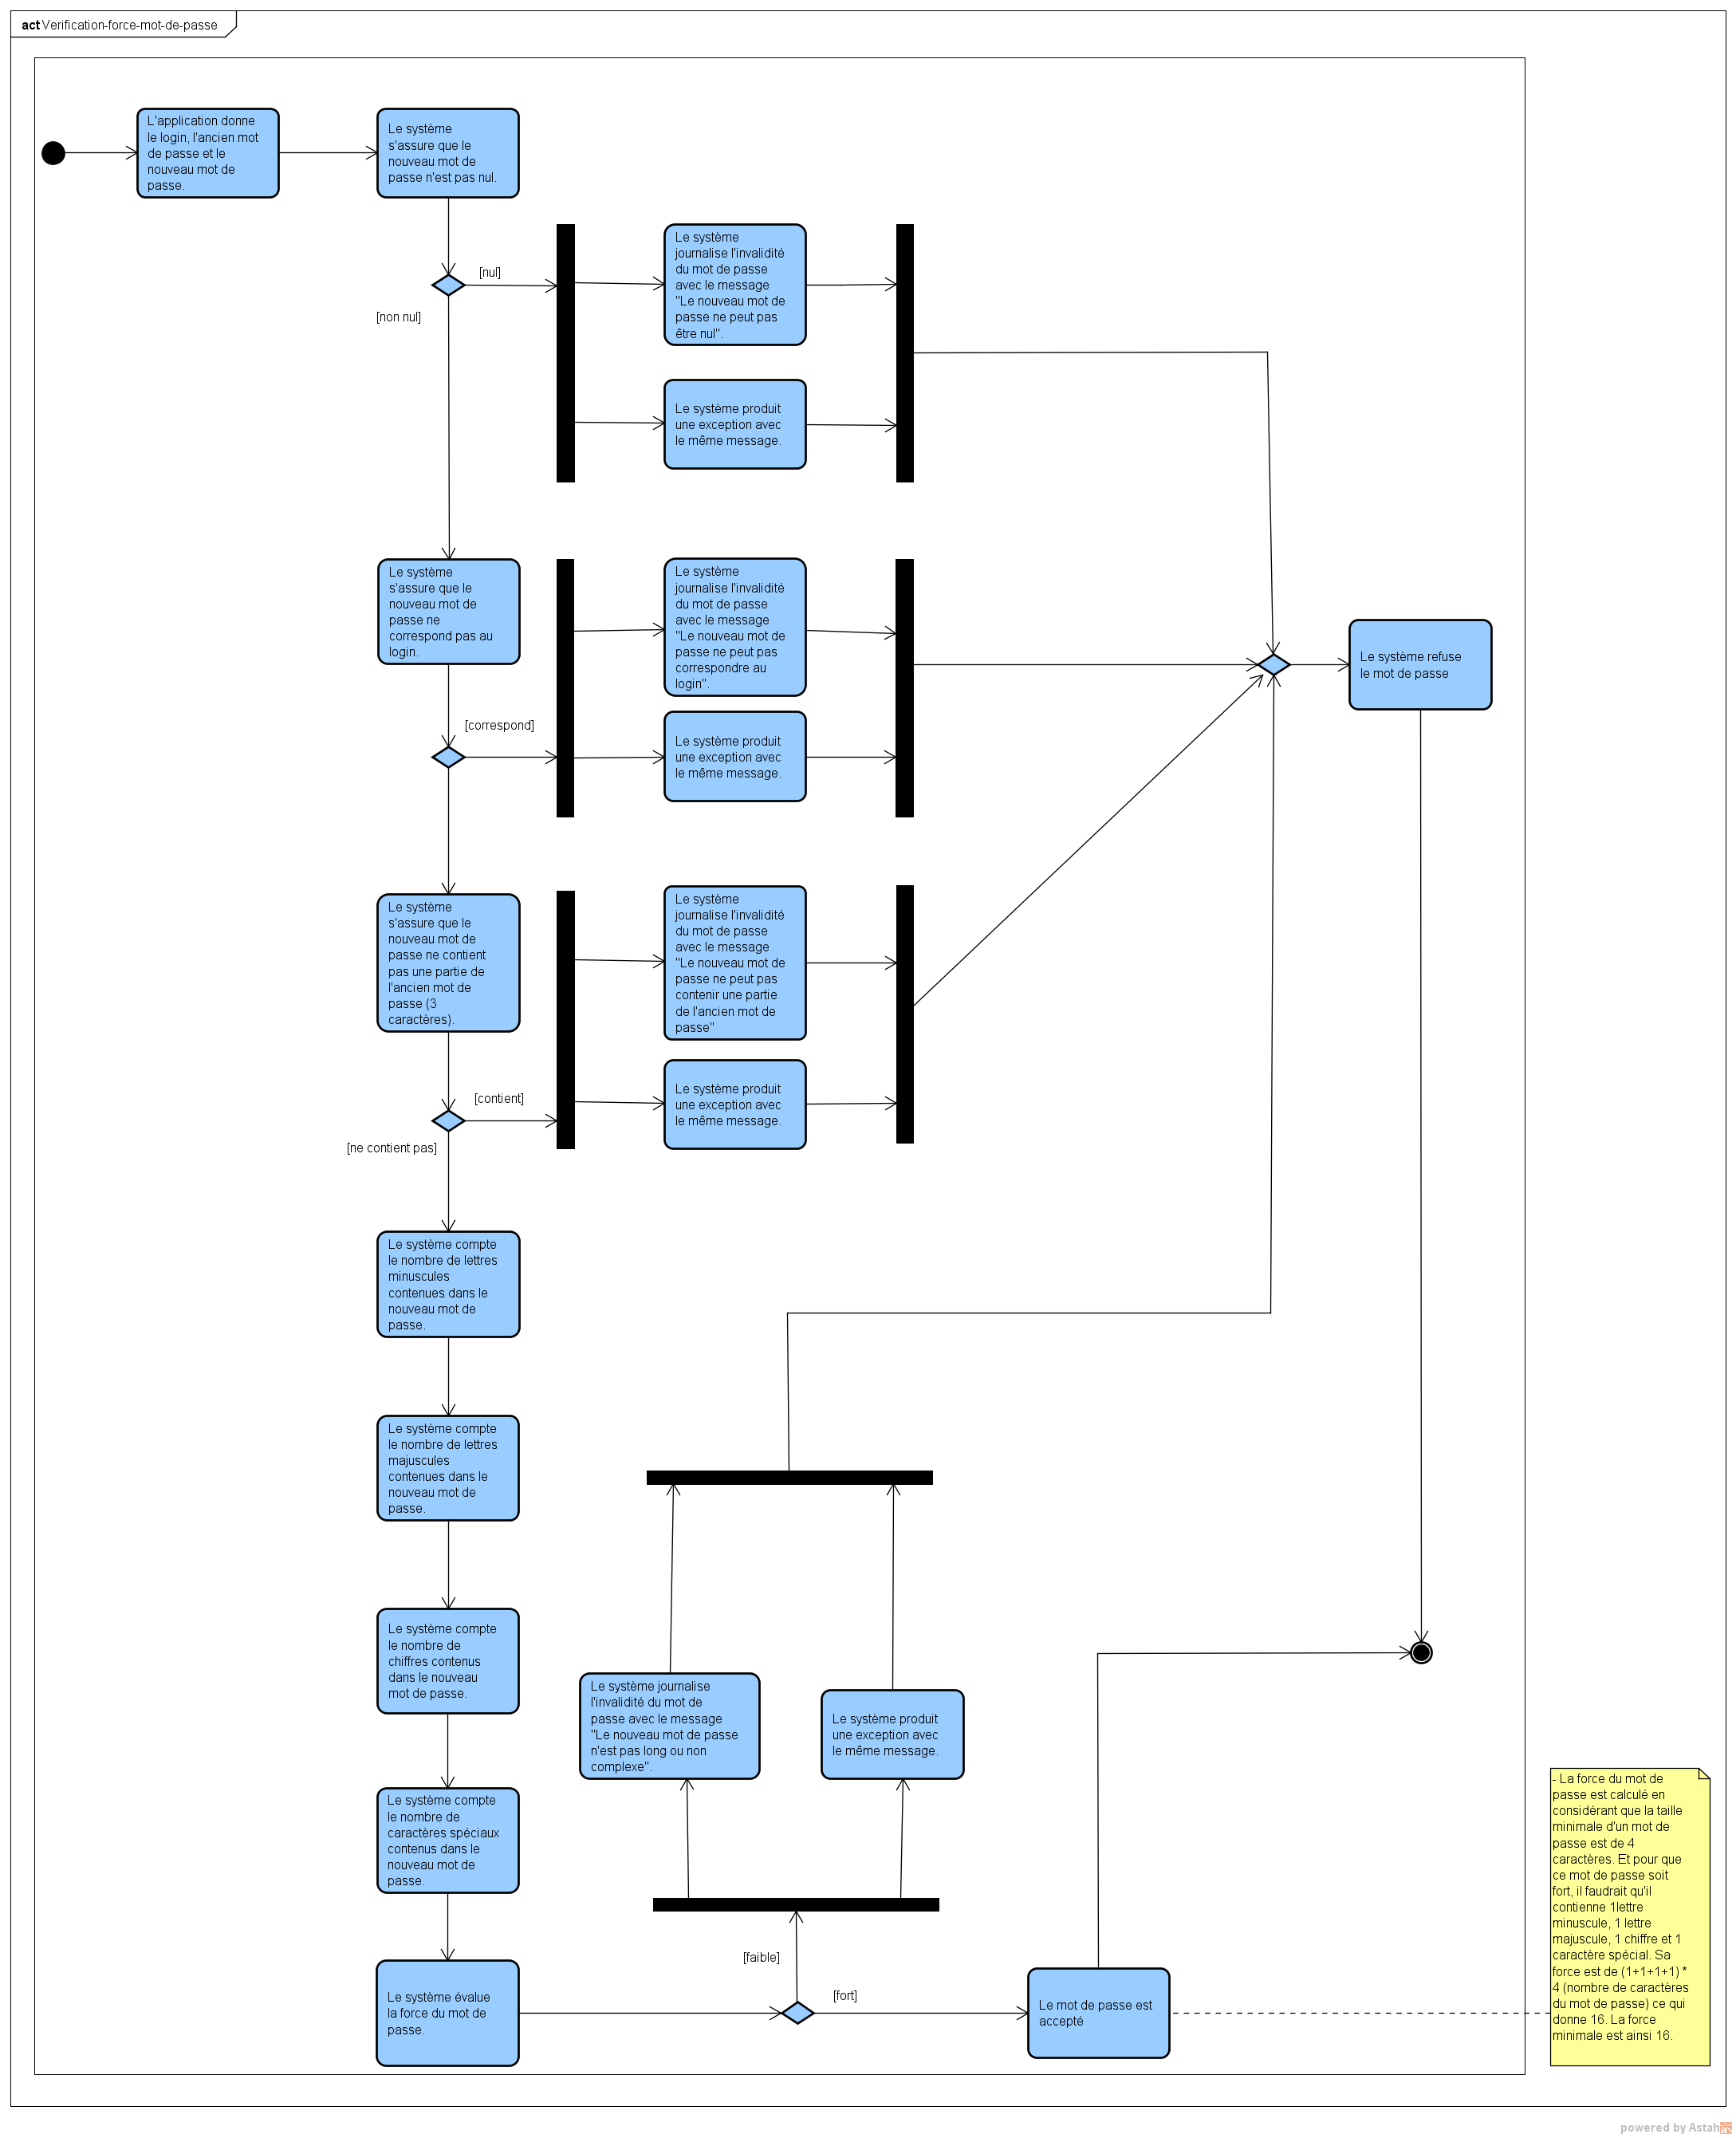
\includegraphics[width=1.0\textwidth,height=0.95\textheight]{fig/Verification-force-mot-de-passe-activity-diagram.png}
	\caption{Diagramme d'activités du cas "Authentification utilisateur"}
\end{figure}

\subsubsection{États d'un utilisateur}
\begin{figure}[H]
	\centering
	\begin{minipage}{12cm}
		\centering
		{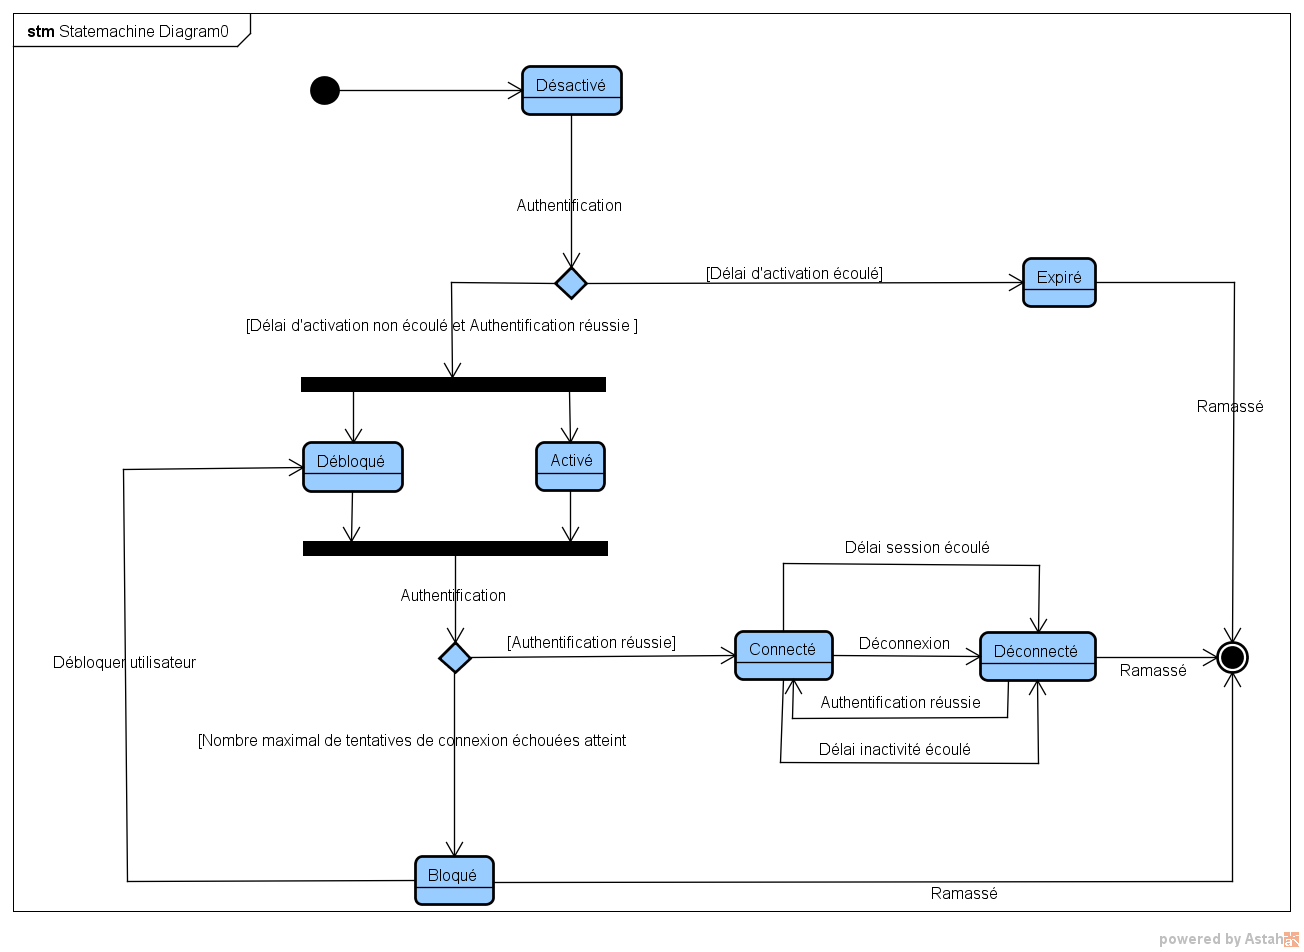
\includegraphics[height=0.35\textheight, width=1\textwidth]{fig/Users-statemachine-diiagram.png}}
	\end{minipage}
	\caption{Diagramme d'états-transition d'un utilisateur}
	\label{fig:7.13}
\end{figure}
%TODO: Petite explication

\subsection{Sous-système "Cryptographie"}
\subsubsection{Diagramme de cas d'utilisation}
\begin{figure}[H]
	\centering
	\begin{minipage}{12cm}
		\centering
		{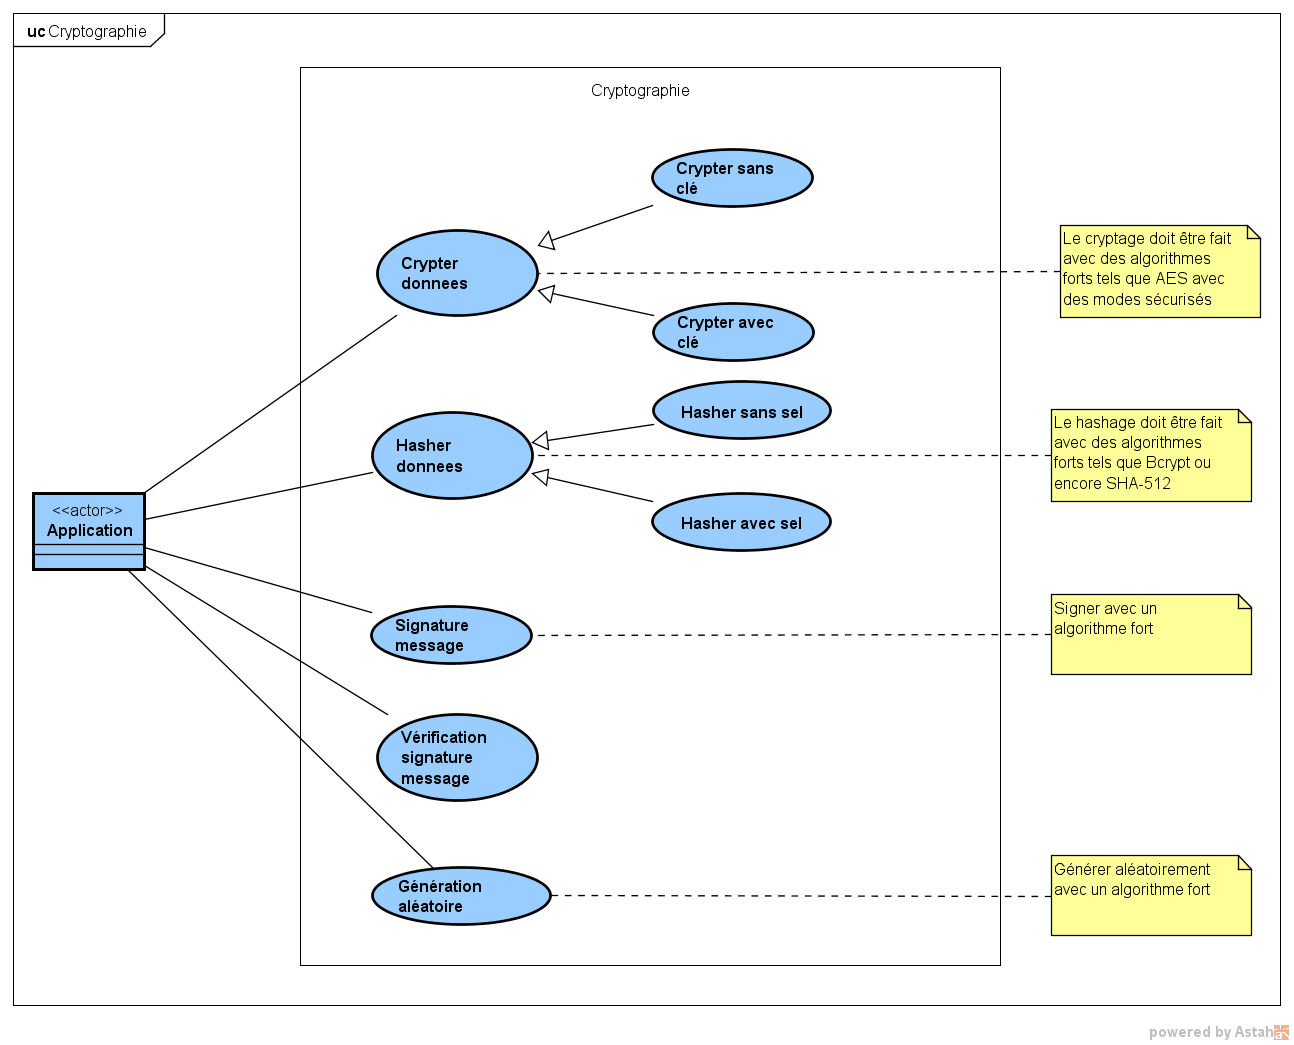
\includegraphics[height=0.35\textheight, width=1\textwidth]{fig/Cryptographie-use-case-diagram.png}}
	\end{minipage}
	\caption{Diagramme de cas d'utilisation du sous-système "Cryptographie"}
	\label{fig:7.14}
\end{figure}
%\subsubsection{Cas d'utilisation "Crypter sans clé"}
*%\textbf{\RIGHTarrow Description textuelle}\\
%\textbf{\RIGHTarrow Diagramme d'activités}\\
%\subsubsection{Cas d'utilisation "Hasher sans sel"}
%\textbf{\RIGHTarrow Description textuelle}\\
%\textbf{\RIGHTarrow Diagramme d'activités}\\

\subsection{Sous-système "Encodage"}
\subsubsection{Diagramme de cas d'utilisation}
\begin{figure}[H]
	\centering
	\begin{minipage}{12cm}
		\centering
		{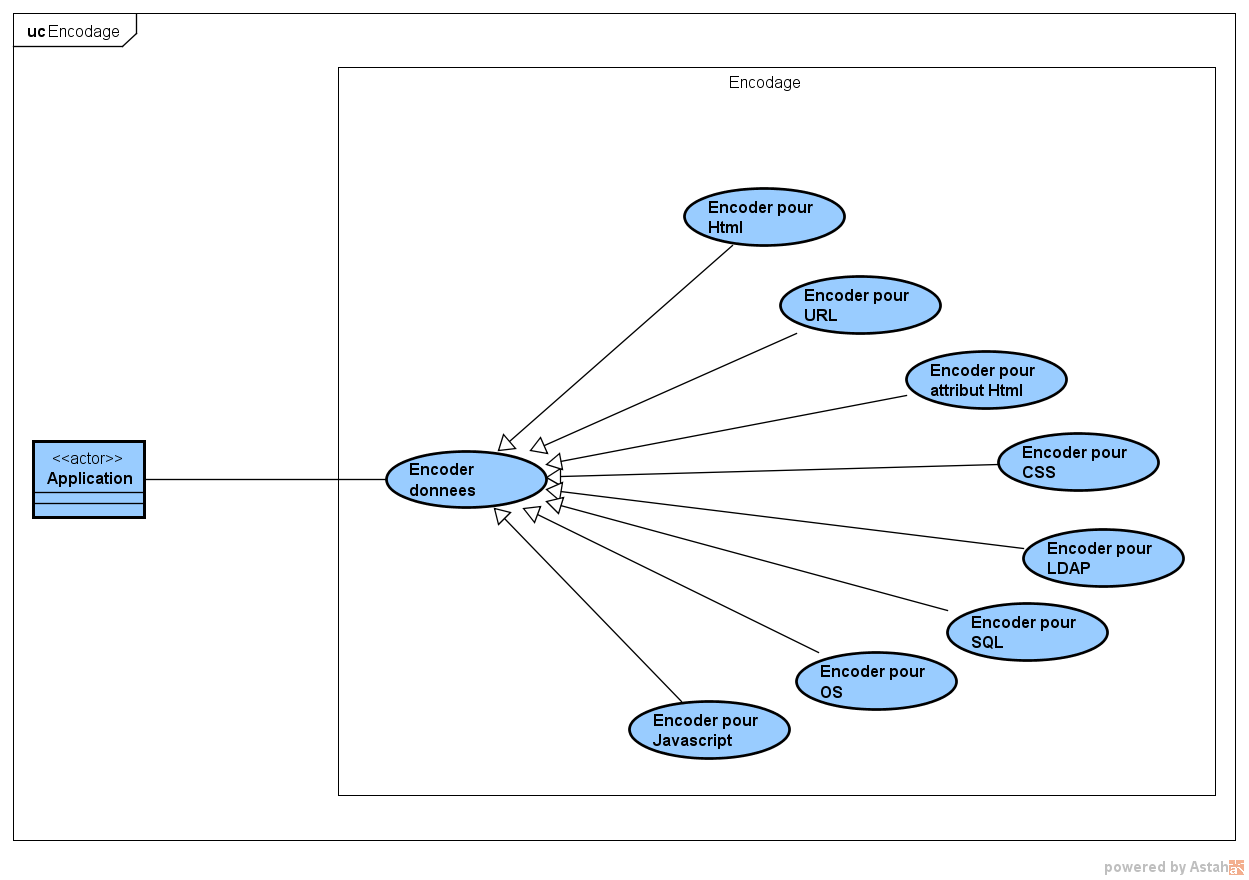
\includegraphics[height=0.35\textheight, width=1\textwidth]{fig/Encodage-use-case-diagram.png}}
	\end{minipage}
	\caption{Diagramme de cas d'utilisation du sous-système "Encodage"}
	\label{fig:7.15}
\end{figure}

\subsection{Sous-système "Validation"}
\subsubsection{Diagramme de cas d'utilisation}
\begin{figure}[H]
	\centering
	\begin{minipage}{12cm}
		\centering
		{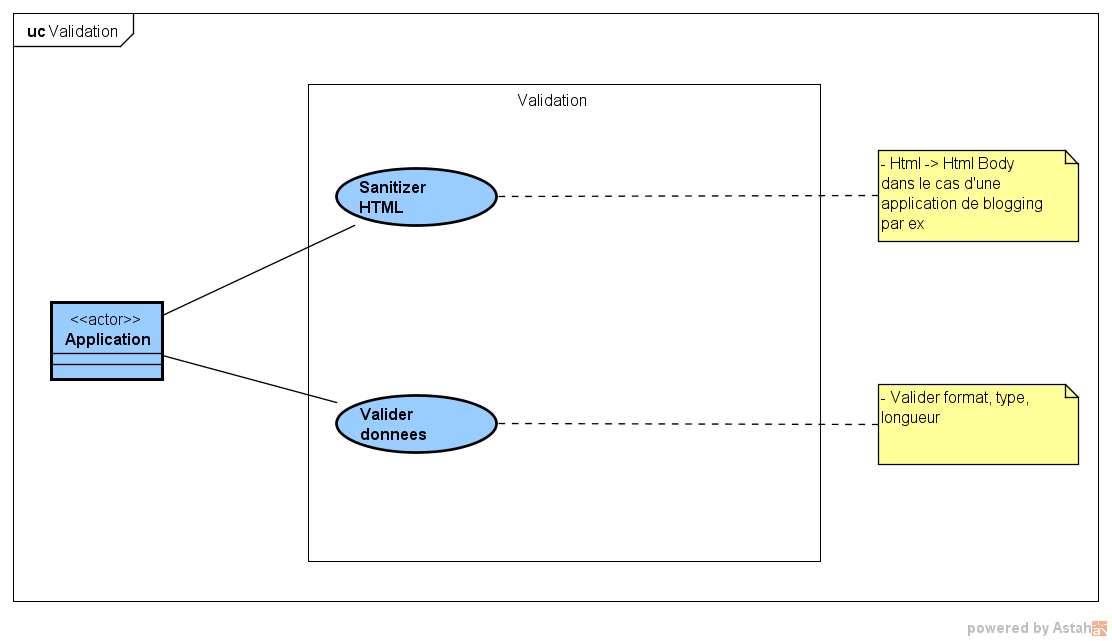
\includegraphics[height=0.35\textheight, width=1\textwidth]{fig/Validation-use-case-diagram.png}}
	\end{minipage}
	\caption{Diagramme de cas d'utilisation du sous-système "Validation"}
	\label{fig:7.16}
\end{figure}
\subsubsection{Cas d'utilisation "Valider donnée"}
\textbf{\RIGHTarrow Description textuelle}\\
\underline{\underline{Sommaire d’identification}} \\
\textbf{Titre} : Valider donnée \\
\textbf{Résumé} : Ce cas d’utilisation permet à une application d'obtenir à partir d'une valeur donnée .\\
\textbf{Acteur} : Application\\	
\textbf{Responsable} : Papa Latyr Mbodj\\
\underline{\underline{Description des scénarios}}\\
\textbf{Précondition(s)}
\begin{itemize}
	\item Aucune
\end{itemize}
\textbf{Scénario nominal}
\begin{enumerate}
	\item L'application donne le login, l'ancien mot de passe et le nouveau mot de passe.
	\item Le système s'assure que le nouveau mot de passe n'est pas nul.
	\item Le système s'assure que le nouveau mot de passe ne correspond pas au login.
	\item Le système s'assure que le nouveau mot de passe ne contient pas une partie de l'ancien mot de passe (3 caractères).
	\item Le système compte le nombre de lettres minuscules contenues dans le nouveau mot de passe.
	\item Le système compte le nombre de lettres majuscules contenues dans le nouveau mot de passe.
	\item Le système compte le nombre de chiffres contenus dans le nouveau mot de passe.
	\item Le système compte le nombre de caractères spéciaux contenus dans le nouveau mot de passe.
	\item Le système évalue la force du mot de passe.
	\item Le mot de passe est accepté.
\end{enumerate}
%\textbf{Enchainements alternatif(s)}\\
\textbf{Enchainements d’erreur}\\
\textit{E1 : Nouveau mot de passe nul}\\
L’enchaînement E1 démarre au point 2 du scénario nominal.
\begin{itemize}
	\item[3.] Le système journalise l'invalidité du mot de passe avec le message "Le nouveau mot de passe ne peut pas être nul".
	\item[4.] Le système produit une exception avec le même message.
	\item[5.] Le système refuse le mot de passe; le cas d'utilisation se termine en échec.
\end{itemize}
\textit{E2 : Nouveau mot de passe correspondant au login}\\
L’enchaînement E2 démarre au point 3 du scénario nominal.
\begin{itemize}
	\item[4.] Le système journalise l'invalidité du mot de passe avec le message "Le nouveau mot de passe ne peut pas correspondre au login".
	\item[5.] Le système produit une exception avec le même message.
	\item[6.] Le système refuse le mot de passe; le cas d'utilisation se termine en échec.
\end{itemize}
\textit{E3 : Nouveau mot de passe contenant une partie de l'ancien mot de passe}\\
L’enchaînement E3 démarre au point 4 du scénario nominal.
\begin{itemize}
	\item[5.] Le système journalise l'invalidité du mot de passe avec le message "Le nouveau mot de passe ne peut pas contenir une partie de l'ancien mot de passe".
	\item[6.] Le système produit une exception avec le même message.
	\item[7.] Le système refuse le mot de passe; le cas d'utilisation se termine en échec.
\end{itemize}
\textit{E4 : Mot de passe faible}\\
L’enchaînement E4 démarre au point 9 du scénario nominal.
\begin{itemize}
	\item[10.] Le système journalise l'invalidité du mot de passe avec le message "Le nouveau mot de passe n'est pas long ou non complexe".
	\item[11.] Le système produit une exception avec le même message.
	\item[12.] Le système refuse le mot de passe; le cas d'utilisation se termine en échec.
\end{itemize}
\textbf{Post-condition(s)}
\begin{itemize}
	\item Le nouveau mot de passe est accepté.
\end{itemize}
\underline{\underline{Exigences non fonctionnelles}}
\begin{itemize}
	\item L’application doit définir une bonne politique de mots de passe.\\
\end{itemize}
\textbf{\RIGHTarrow Diagramme d'activités}\\

\subsection{Sous-système "HTTP"}
\subsubsection{Diagramme de cas d'utilisation}
\begin{figure}[H]
	\centering
	\begin{minipage}{12cm}
		\centering
		{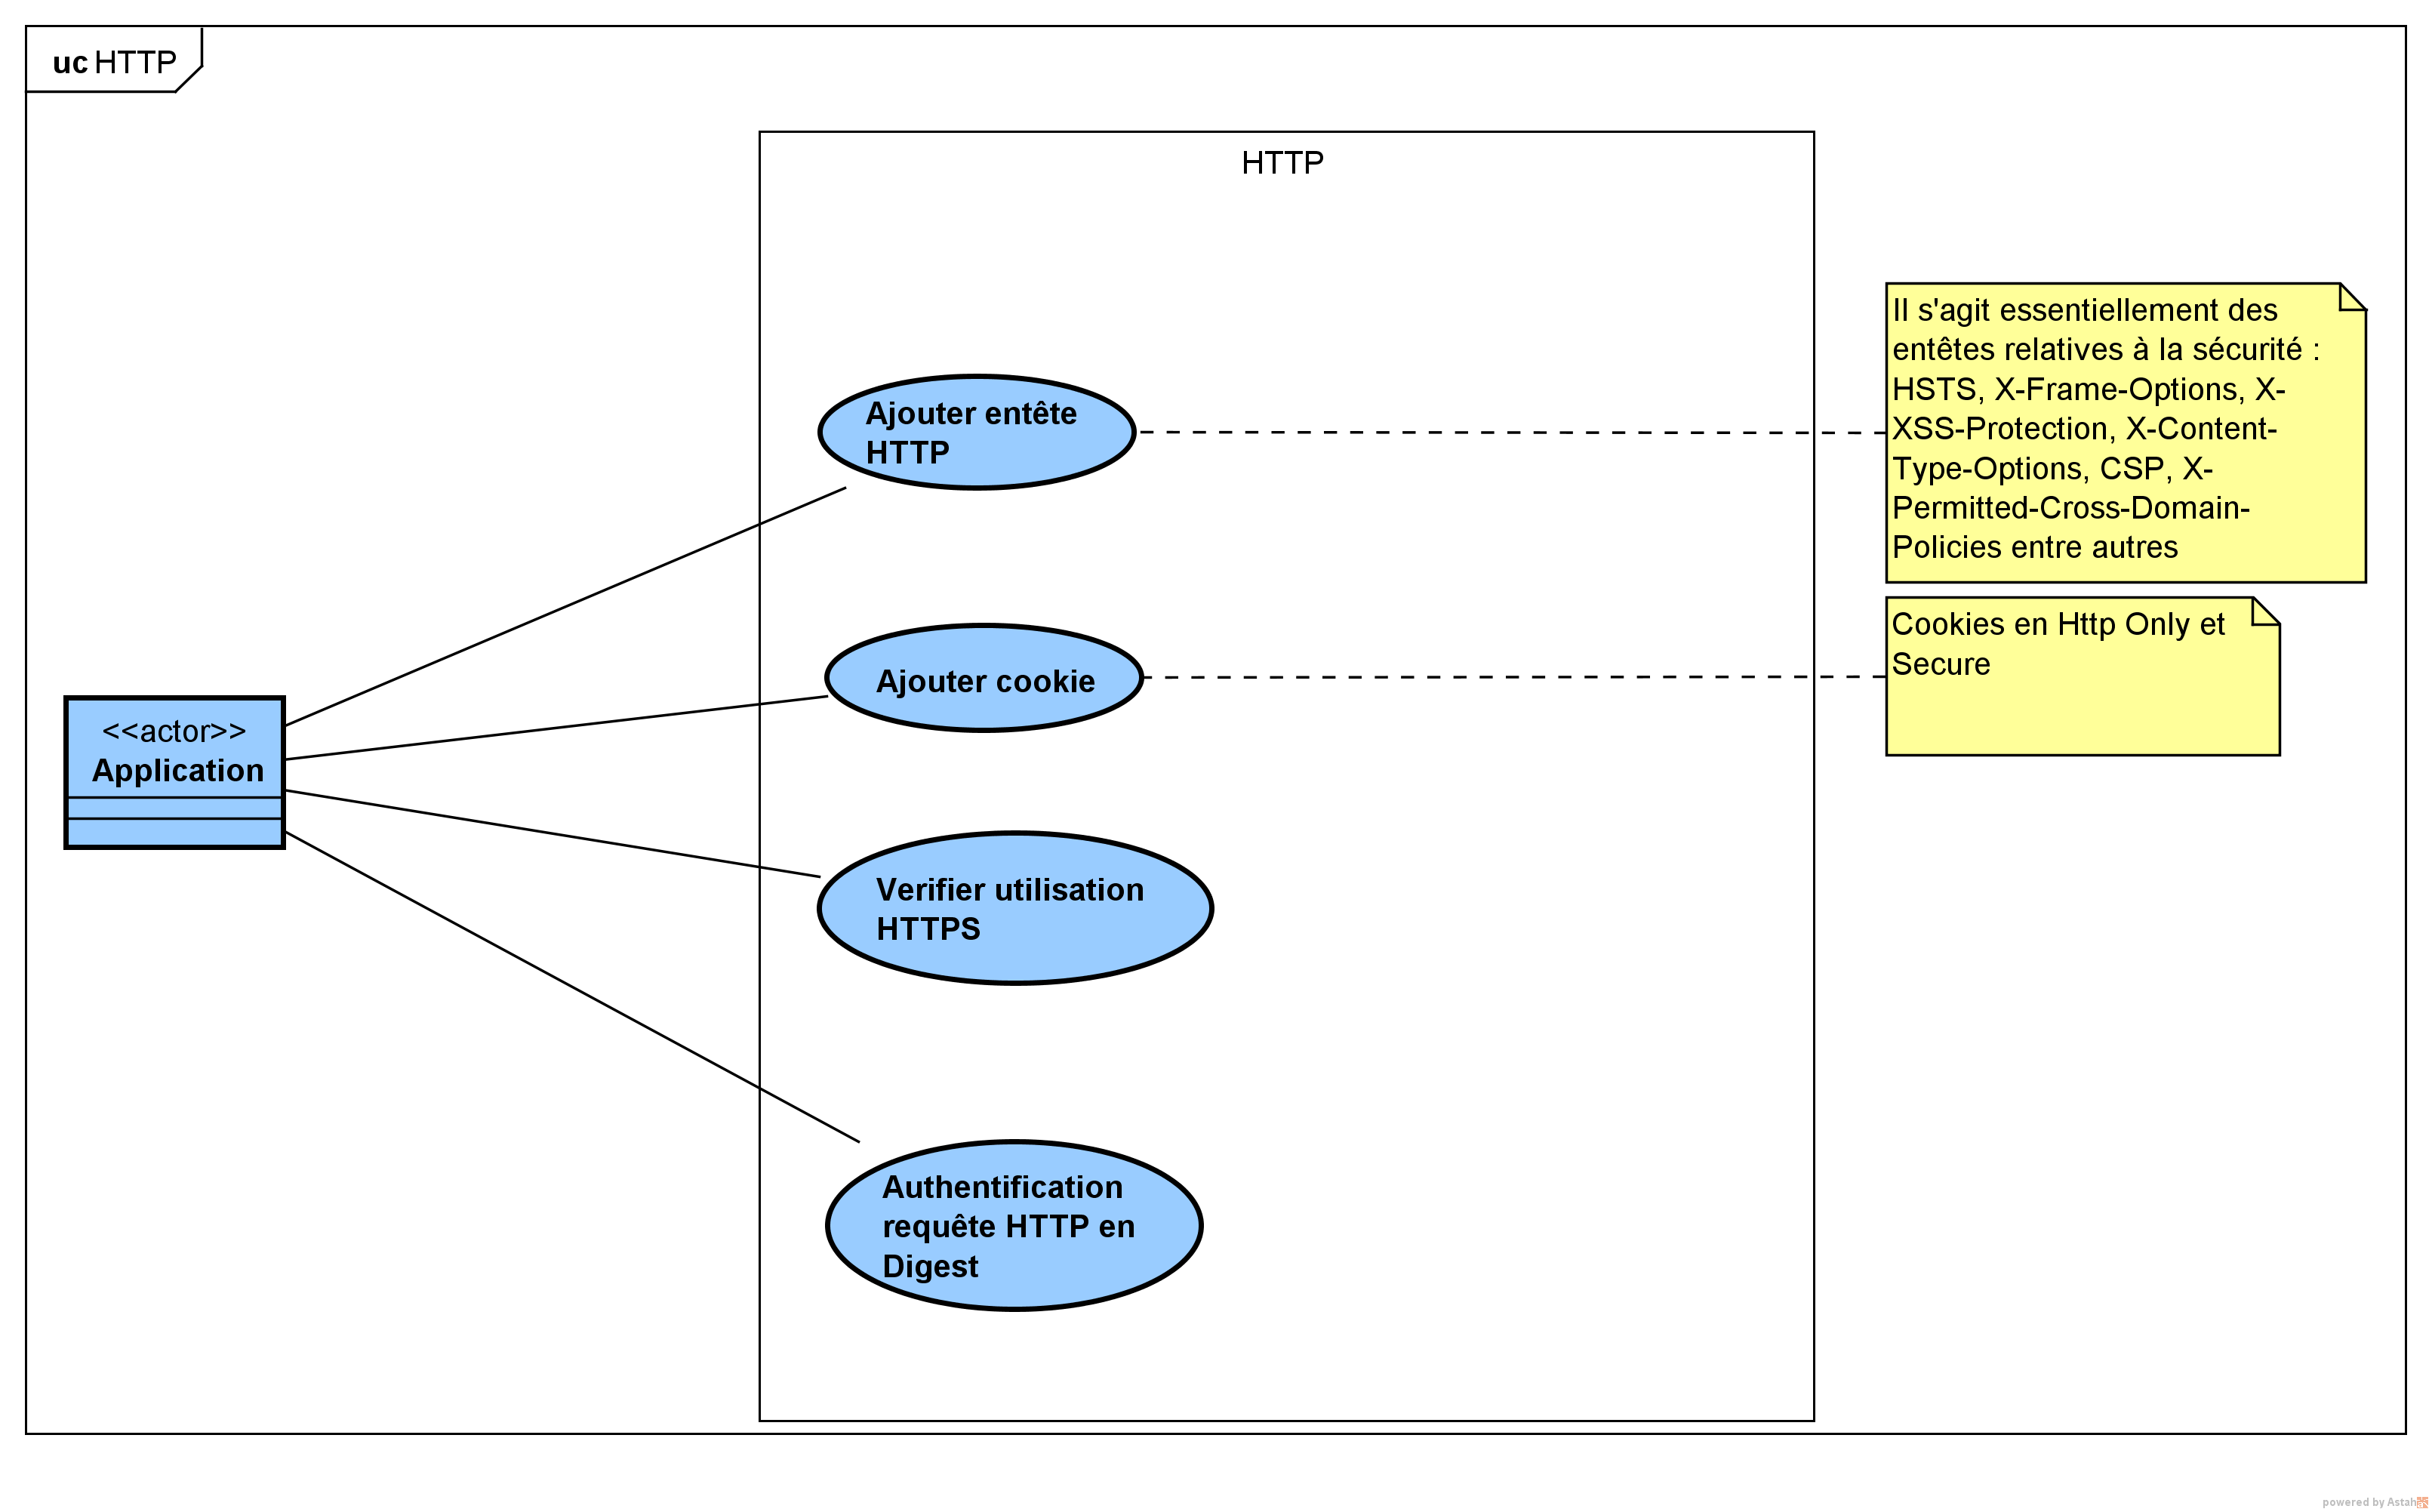
\includegraphics[height=0.35\textheight, width=1\textwidth]{fig/HTTP-use-case-diagram.png}}
	\end{minipage}
	\caption{Diagramme de cas d'utilisation du sous-système "HTTP"}
	\label{fig:7.17}
\end{figure}
\subsubsection{Cas d'utilisation "Ajouter cookie"}
\textbf{\RIGHTarrow Description textuelle}\\
\textbf{\RIGHTarrow Diagramme d'activités}\\
%\subsubsection{Cas d'utilisation "Authentification requête HTTP en  Digest"}
%\textbf{\RIGHTarrow Description textuelle}\\
%\textbf{\RIGHTarrow Diagramme d'activités}\\

\subsection{Sous-système "Interpréteurs"}
\subsubsection{Diagramme de cas d'utilisation}
\begin{figure}[H]
	\centering
	\begin{minipage}{12cm}
		\centering
		{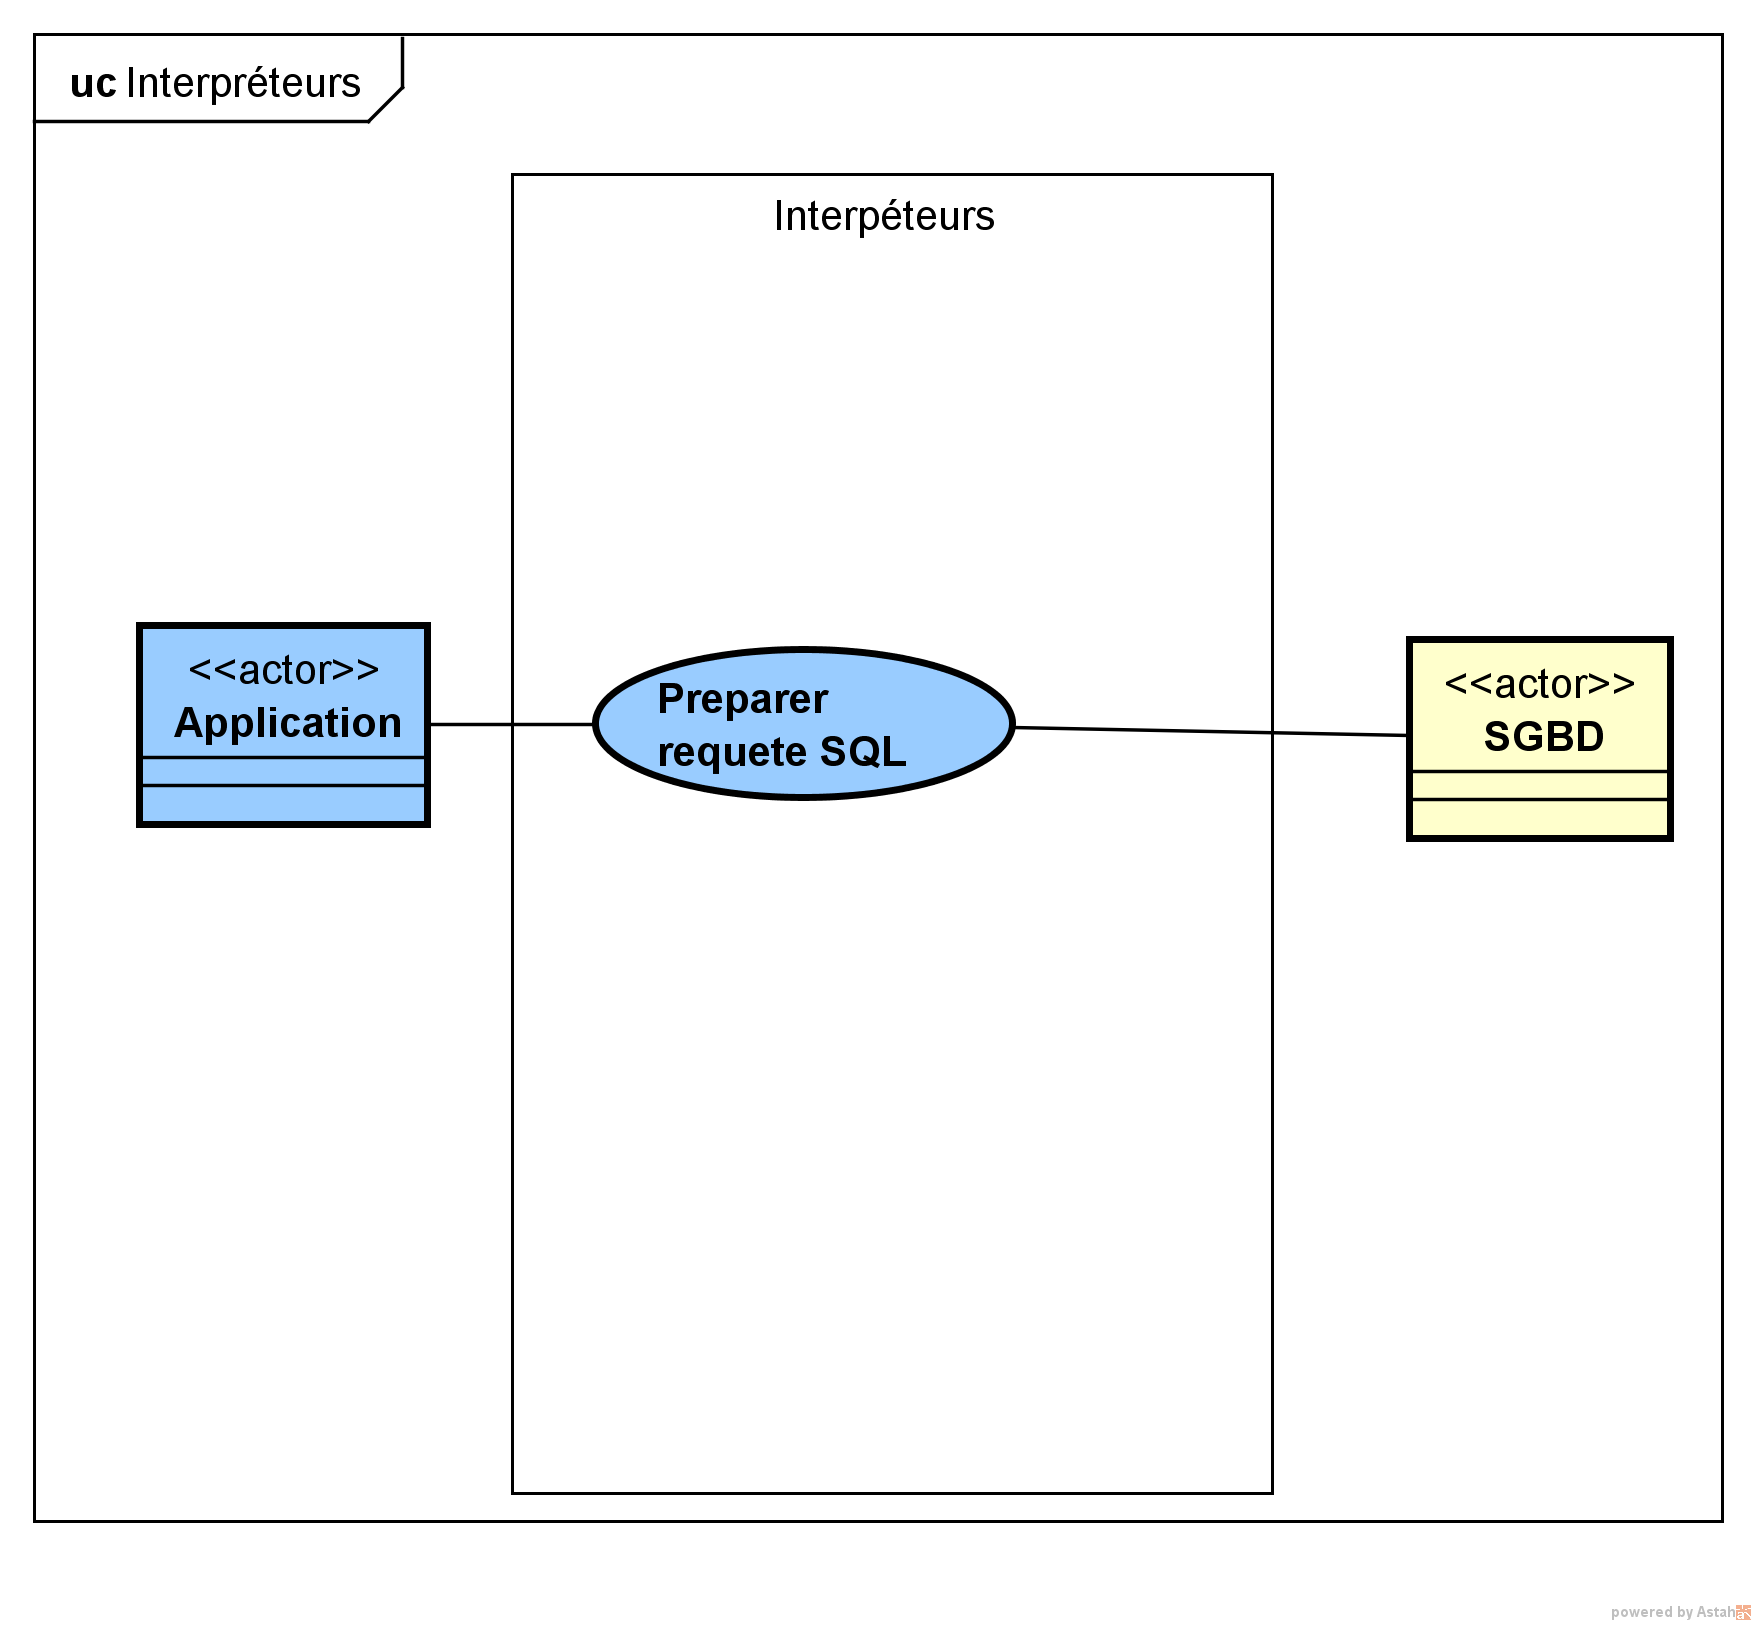
\includegraphics[height=0.3\textheight, width=1\textwidth]{fig/Interpreteurs-use-case-diagram.png}}
	\end{minipage}
	\caption{Diagramme de cas d'utilisation du sous-système "Interpreteurs"}
	\label{fig:7.18}
\end{figure}


\subsection{Sous-système "Logging"}
\subsubsection{Diagramme de cas d'utilisation}
\begin{figure}[H]
	\centering
	\begin{minipage}{12cm}
		\centering
		{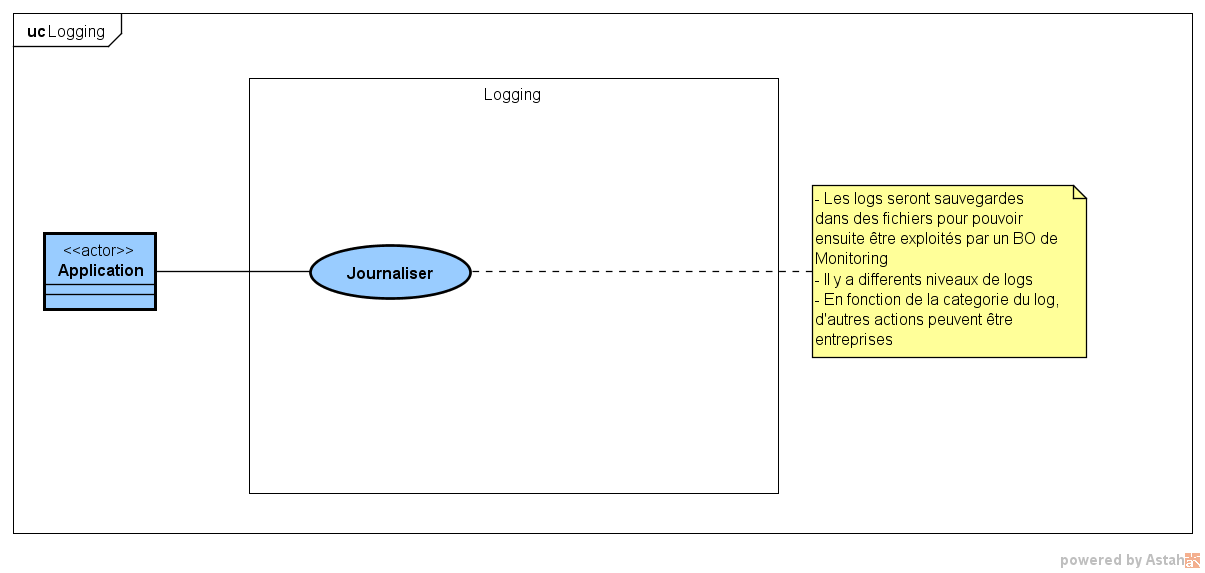
\includegraphics[height=0.35\textheight, width=1\textwidth]{fig/Logging-use-case-diagram.png}}
	\end{minipage}
	\caption{Diagramme de cas d'utilisation du sous-système "Gestion de la journalisation et de la surveillance insuffisantes"}
	\label{fig:7.19}
\end{figure}

\subsection{Sous-système "Gestion des composants"}
\subsubsection{Diagramme de cas d'utilisation}
\begin{figure}[H]
	\centering
	\begin{minipage}{12cm}
		\centering
		{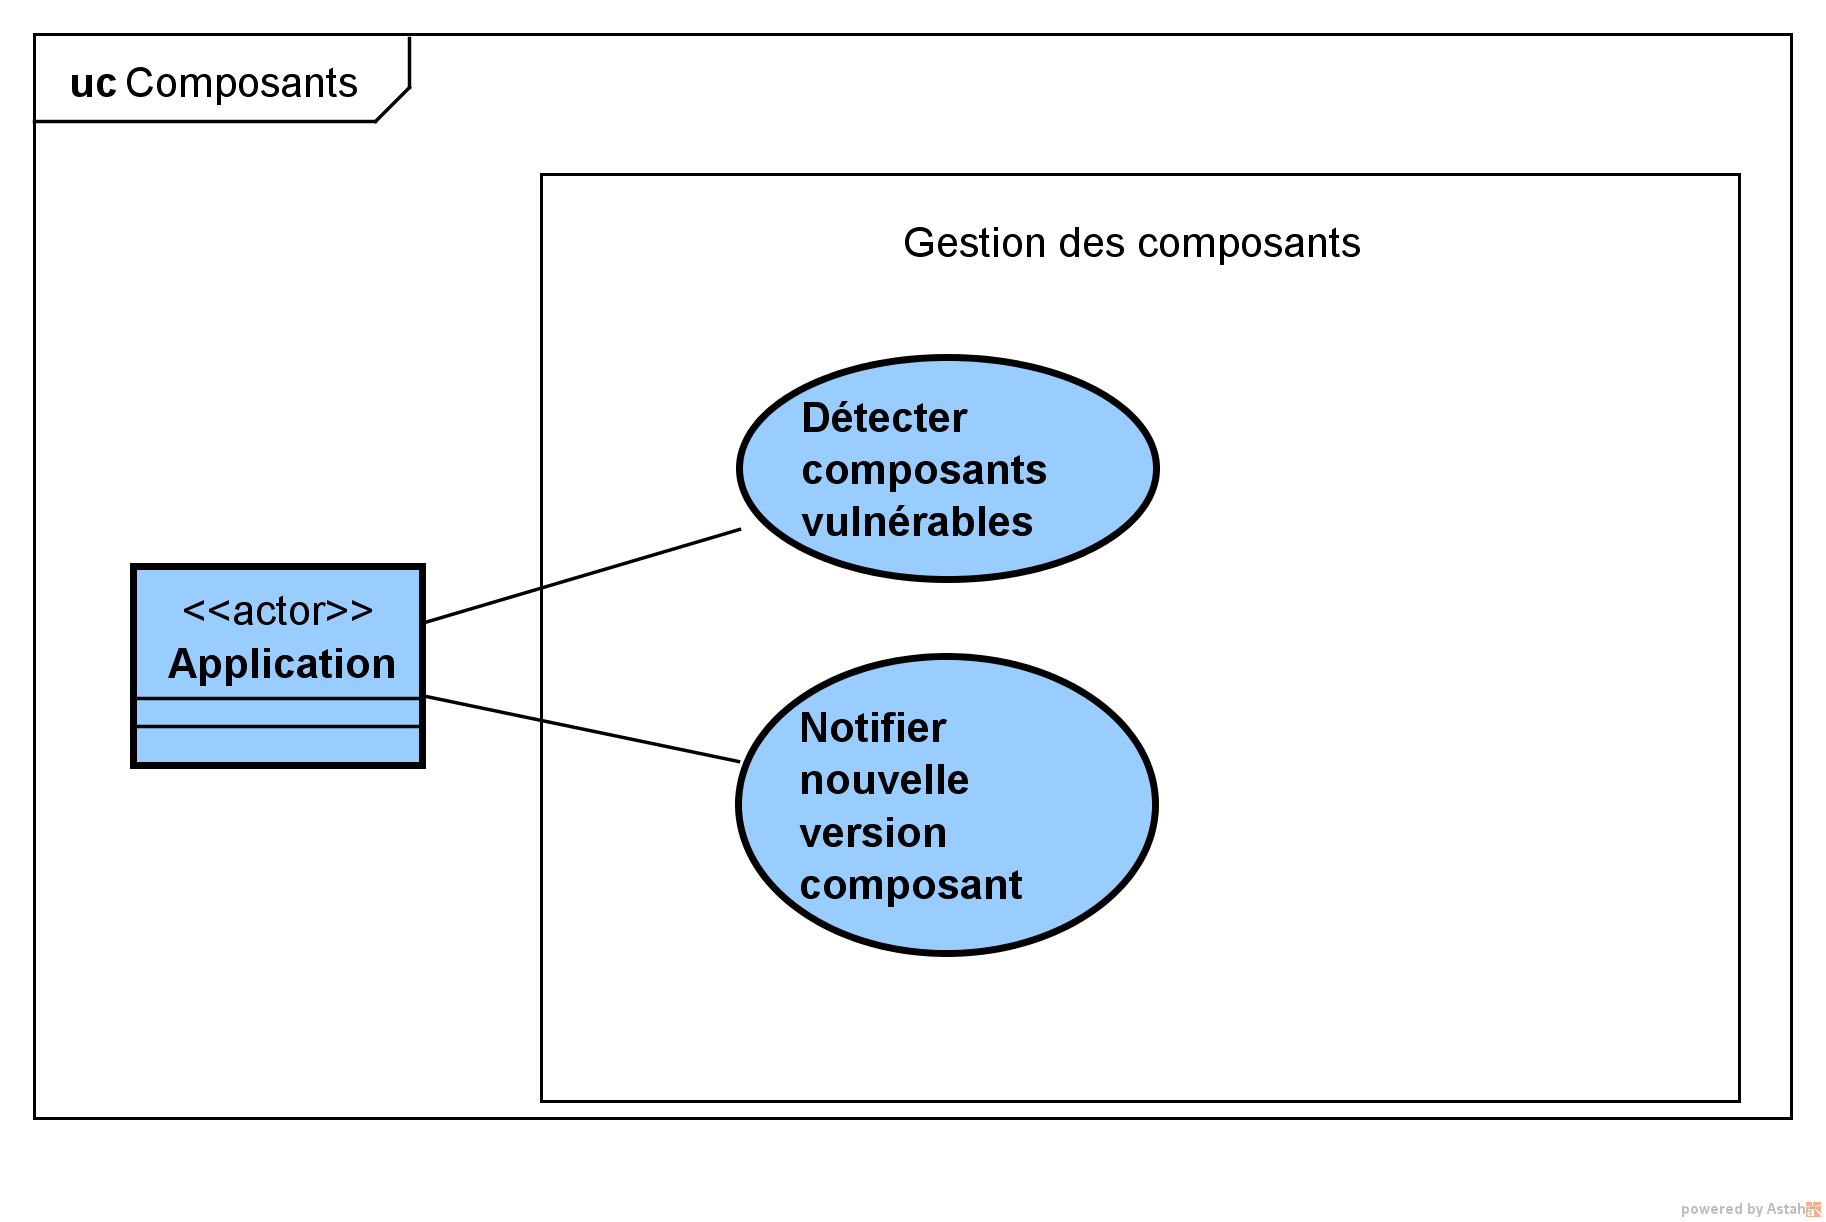
\includegraphics[height=0.35\textheight, width=1\textwidth]{fig/Composants-use-case-diagram.png}}
	\end{minipage}
	\caption{Diagramme de cas d'utilisation du sous-système "Gestion de la journalisation et de la surveillance insuffisantes"}
	\label{fig:7.20}
\end{figure}
%\subsubsection{Cas d'utilisation "Détecter composants vulnérables"}
%\textbf{\RIGHTarrow Description textuelle}\\
%\textbf{\RIGHTarrow Diagramme d'activités}\\
\subsection{Diagramme de classes}
\begin{figure}[H]
	\centering
	\begin{minipage}{12cm}
		\centering
		{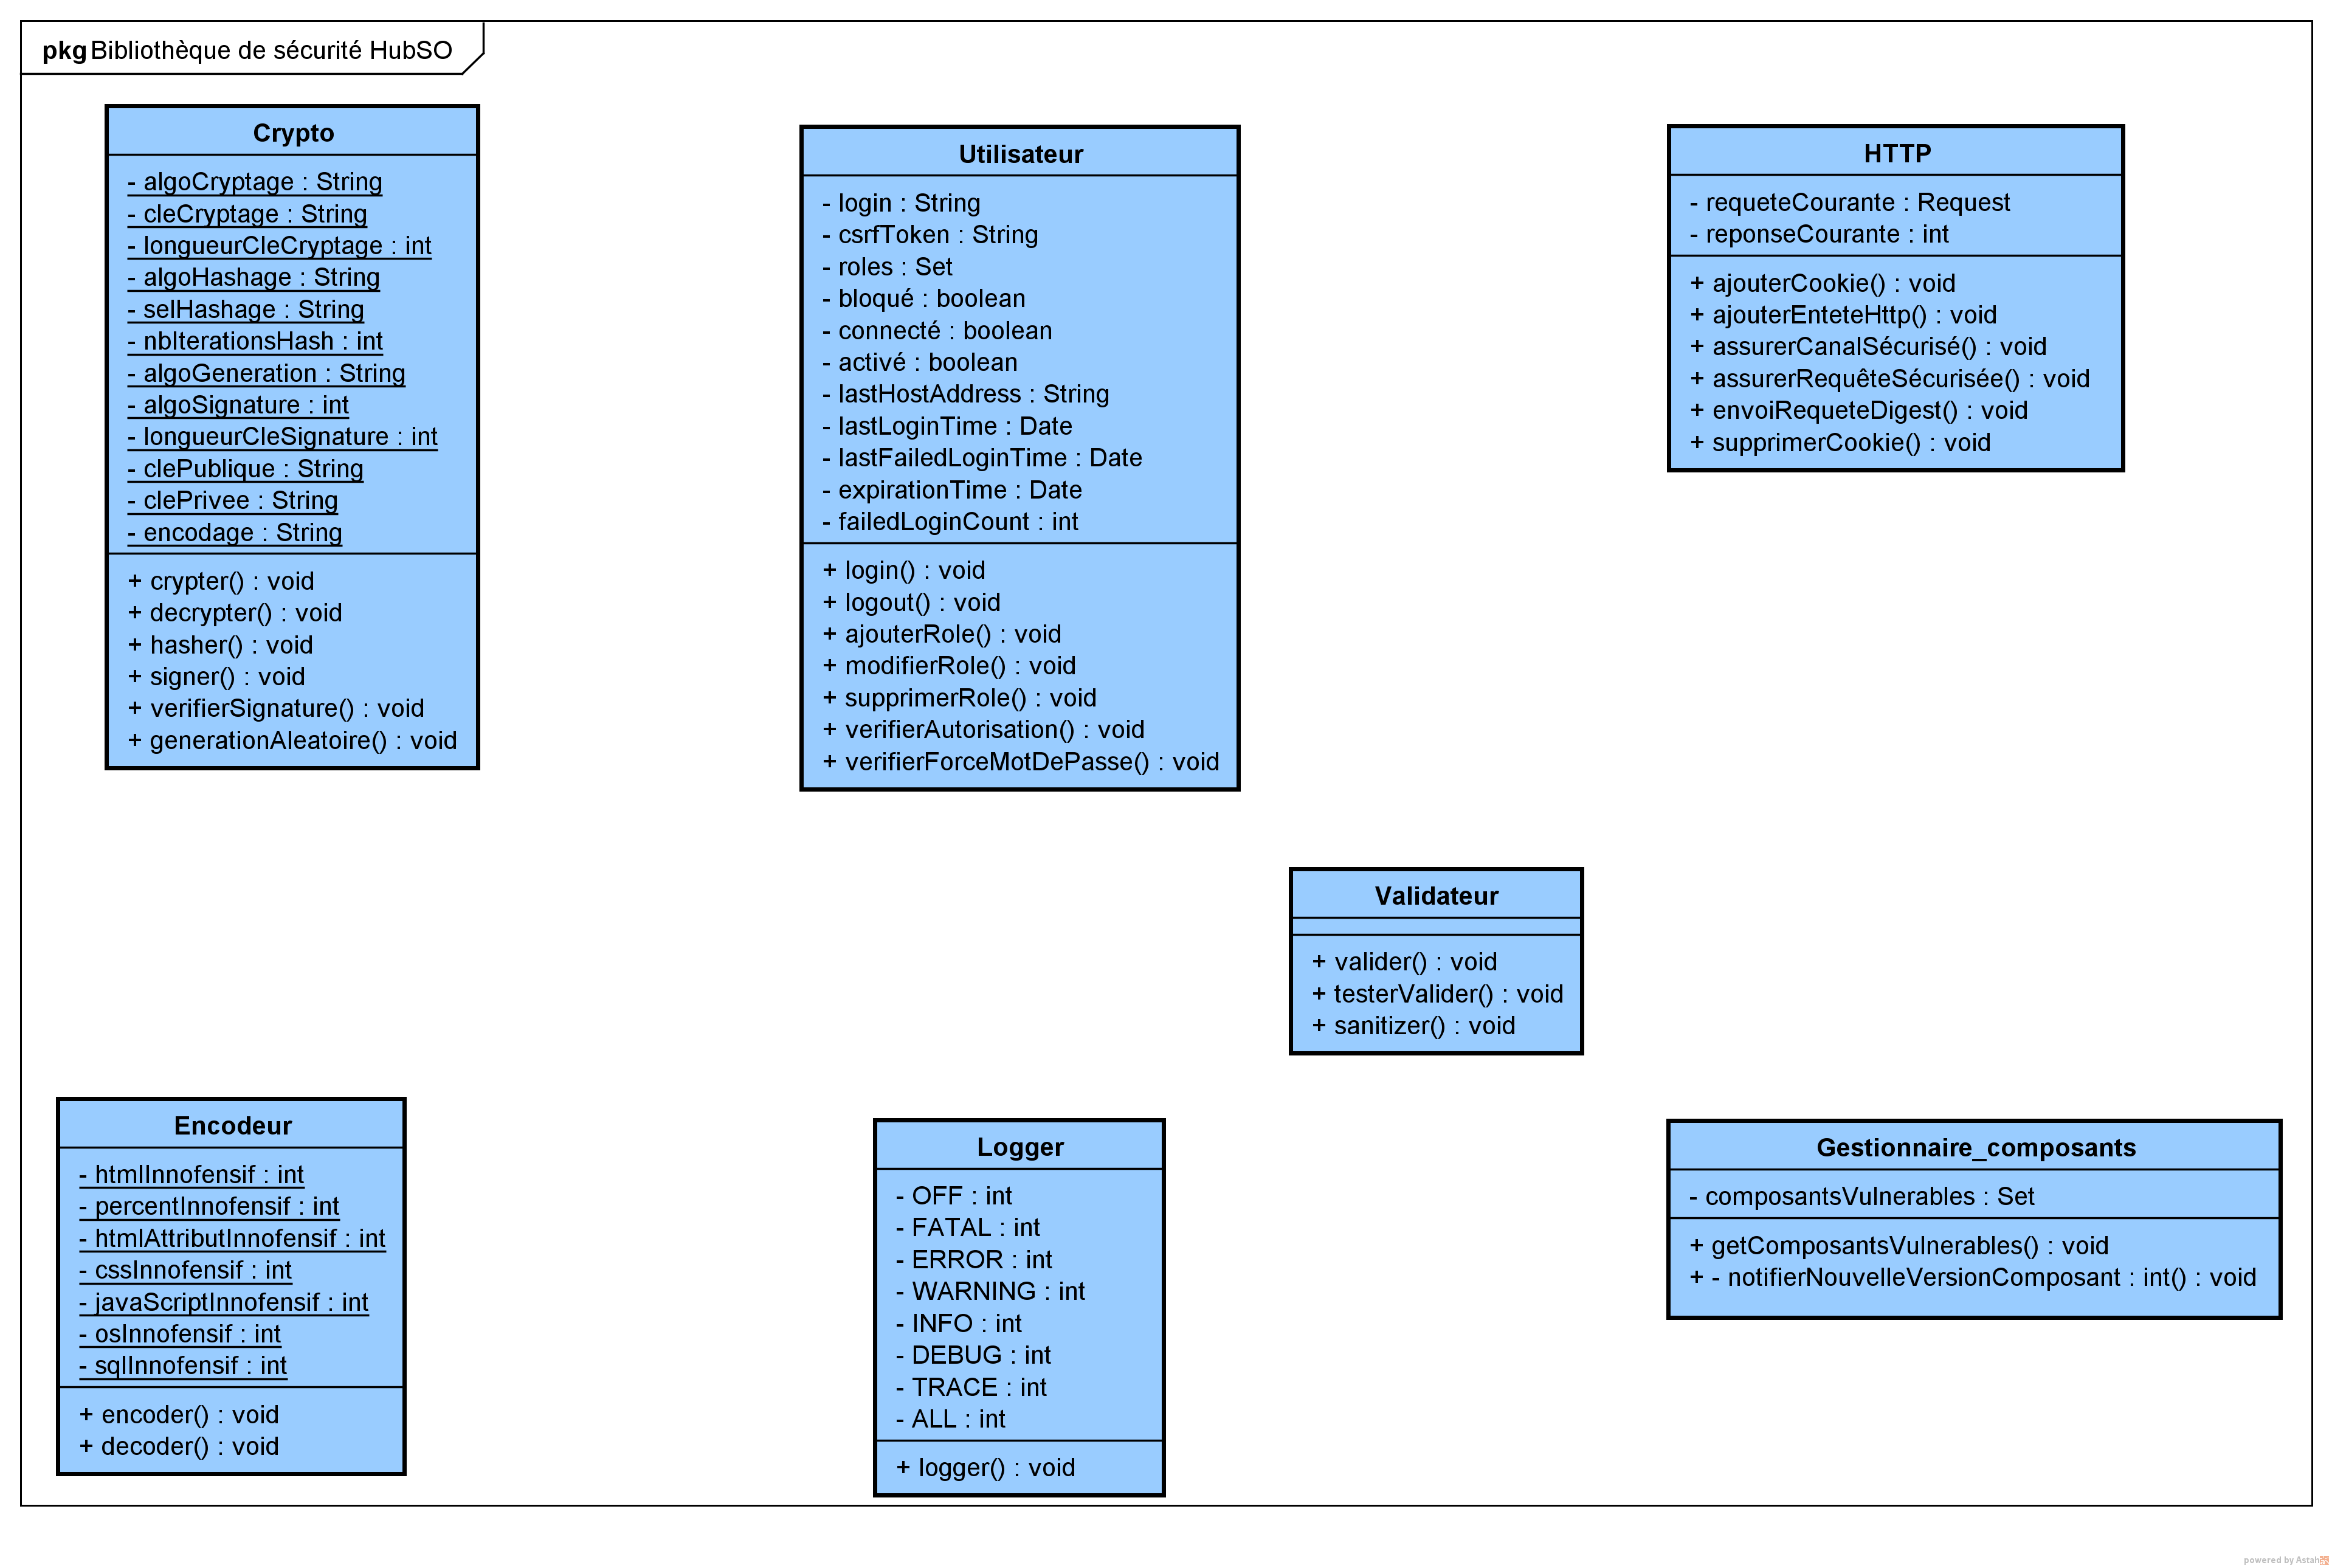
\includegraphics[height=0.35\textheight, width=1\textwidth]{fig/Analyse-Class-Diagram.png}}
	\end{minipage}
	\caption{Diagramme de classes d'analyse dy système}
	\label{fig:7.20}
\end{figure}

\section{Conception}
\subsection{Architecture Technique}
L’architecture désigne la structure générale inhérente à un système informatique, l'organisation des différents éléments du système et des relations entre les éléments. Cette structure fait suite à un ensemble de décisions stratégiques prises durant la conception de tout ou une partie du système.\\
L´architecture technique est une vue tournée vers les différents éléments matériels et l'infrastructure dans laquelle le système informatique s'inscrit, les liaisons physiques et logiques entre ces éléments et les informations qui y circulent.https://fr.wikipedia.org/wiki/Architecture_(informatique)\\
L'architecture d'une application Web ou Mobile joue aussi un rôle très important dans la sécurité de ces applications. En effet, une bonne architecture représente déjà une bonne défense. Owasp pr
L’architecture du système est une architecture de type 3-tiers :
Un serveur d’application gérant la logique métier de l’application.
Un serveur web qui gère la communication entre le serveur d’application et le navigateur.
Un serveur de base de données gérant la base de données de l’application.
Ces trois composants seront installés dans des machines virtuelles différentes qui représentent les services du cloud.
Un pare-feu1est mis en place pour filtrer les connexions entrantes et sortantes. Les services Web sont utilisés pour intégrer d’autres applications avec le système.
Les utilisateurs finaux accèdent au système par le biais d’un navigateur.
\subsection{Diagramme de déploiement}

\subsection{La bibliothèque ESAPI}
Allowing for language-specific differences, all OWASP ESAPI versions have the
same basic design:
 There is a set of security control interfaces. There is no application logic
contained in these interfaces. They define for example types of parameters
that are passed to types of security controls. There is no proprietary
information or logic contained in these interfaces.
 There is a reference implementation for each security control. There is
application logic contained in these classes, i.e. contained in these interface
implementations. However, the logic is not organization-specific and the
logic is not application-specific. There is no proprietary information or
logic contained in these reference implementation classes. An example:
string-based input validation.
 There are optionally your own implementations for each security control.
There may be application logic contained in these classes which may be
developed by or for your organization. The logic may be organizationspecific
and/or application-specific. There may be proprietary
information or logic contained in these classes which may be developed
by or for your organization. An example: enterprise authentication.
There are three common ways to write your own implementations for each 
Après avoir fini la phase d'analyse, nous passons maintenant à la phase de conception
Why you shouldn’t build your own security controls
Writing security controls is time-consuming and extremely prone to mistakes. MITRE’s CWE project lists
over 600 different types of security mistakes that developers can make, and most of them are not at all
obvious. Most people recognize that developers should not build their own encryption mechanisms, but
the same argument applies to all the security controls. 
Why you shouldn’t use security libraries directly
There are plenty of libraries and frameworks out there that provide various security functions – Log4j,
Java Cryptographic Extension (JCE), JAAS, Acegi, and dozens more. Some of them are even pretty good
at what they do. But there are several reasons why enterprise developers should not use them directly.
Most importantly, these libraries are overpowerful. Most developers only need a very limited set of
security functions and don’t need a complex interface. Further, many of these libraries contain security
holes themselves – such as encoding libraries that don’t canonicalize or authentication libraries that
don’t use strong cryptographic functions. Because many security controls use features from other
controls, using security libraries that aren’t integrated together is a mistake.
Why you shouldn’t rely on security in the platform or framework
Unfortunately, the web application platforms and frameworks do not protect against many well-known
attacks. For example, consider header injection – allowing carriage return (CR) and line-feed (LF)
characters to be used in HTTP headers. This injection changes the way these HTTP messages are parsed,
allowing the attacker to affect how they are interpreted. This type of injection can allow attackers to
download malicious files to the user’s desktop among other serious impacts.
The platforms could protect against this attack which violates the HTTP specification, but many do not.
Instead, your application developers must know to carefully validate and filter user data before using it
in HTTP headers.
The platforms and frameworks are a shifting environment. Your code may be protected by something in
your infrastructure today, but that environment may change tomorrow. The best approach is to build
your applications so that they provide their own protection. If this results in some overlapping
protection, also known as defense-in-depth, that’s a good outcome. 

Interfaces
ESAPI is primarily a set of interfaces designed to make security easy to use. These interfaces are usable
by anyone who cares to implement them for their enterprise. By keeping the interfaces separate, we are
trying to encourage organizations to create their own implementations.
However, we didn’t stop there. We built a complete set of reference implementations. The reference
implementations are complete and well tested, although there are a few limitations. In general, the
reference implementation is designed to run without requiring any other infrastructure, such as
database or LDAP servers.
The Authenticator and AccessController implementations in particular work of simple text file policies,
which may not be appropriate for enterprise applications. However, the rest of the reference
implementation is scalable and appropriate for enterprise applications. You will likely want to hook up
the Logger to your logging infrastructure. 
Assurance
It’s absolutely critical to get your applications security controls right. An error could expose many
applications. Confidence in your security controls comes from evidence like design documentation, code
review, security testing, and other analysis. 

The ESAPI project involves a world-class team of software security experts from vendors and industry.
The reference implementation is small and well structured – about 5,000 lines of well-documented and
extensively reviewed code. The code is clean in all the major static analysis tools, including FindBugs,
PMD, Ounce, and Fortify. The project also includes about 600 test cases that test all aspects of the
security mechanisms. 

\subsubsection{Architecture fonctionnelle}
\subsubsection{Architecture Fonctionnelle détaillée}

\subsection{Diagramme de classes de conception}
